% Author: Victor Terron (c) 2013
% Email: `echo vt2rron1iaa32s | tr 132 @.e`
% License: GNU GPLv3

\documentclass[14pt]{beamer}

\usepackage[utf8]{inputenc}
\usepackage{listings}
\usepackage[T1]{fontenc}

% Reduce space between image and caption; also remove prefix 'Figure:'
% http://tex.stackexchange.com/a/94018
% http://tex.stackexchange.com/a/82462
\usepackage[font=small,skip=1pt,labelformat=empty]{caption}

% New line between paragraphs, no indentation
% http://tex.stackexchange.com/q/42
\usepackage[parfill]{parskip}

\usetheme{Copenhagen}
\useoutertheme{infolines}
\setbeamercovered{dynamic}
\setbeamertemplate{navigation symbols}{} % remove navigation symbols

\lstset{basicstyle=\ttfamily,language=python}

% Remove the space symbol for code inside the double quotation marks
% http://www.latex-community.org/viewtopic.php?f=4&t=248
\lstset{showstringspaces=false}

% Enable accents and ñ in our code listings
% http://stackoverflow.com/a/2782147/184363
\lstset{
  literate={á}{{\'a}}1
           {é}{{\'e}}1
           {í}{{\'i}}1
           {ó}{{\'o}}1
           {ú}{{\'u}}1
           {ñ}{{\~n}}1
           {¡}{{\textexclamdown}}1
}

\definecolor{red}{HTML}{F41B1B}
\definecolor{blue}{HTML}{2E3CEC}
\definecolor{green}{HTML}{3C8031}

% Beamer: footer with current slide number but not total slide number
% http://tex.stackexchange.com/a/32815
\makeatletter
\setbeamertemplate{footline}
{
  \leavevmode%
  \hbox{%
  \begin{beamercolorbox}[wd=.333333\paperwidth,ht=2.25ex,dp=1ex,center]{author in head/foot}%
    \usebeamerfont{author in head/foot}\insertshortauthor~~\beamer@ifempty{\insertshortinstitute}{}{(\insertshortinstitute)}
  \end{beamercolorbox}%
  \begin{beamercolorbox}[wd=.333333\paperwidth,ht=2.25ex,dp=1ex,center]{title in head/foot}%
    \usebeamerfont{title in head/foot}\insertshorttitle
  \end{beamercolorbox}%
  \begin{beamercolorbox}[wd=.333333\paperwidth,ht=2.25ex,dp=1ex,right]{date in head/foot}%
    \usebeamerfont{date in head/foot}\insertshortdate{}\hspace*{2em}
    \insertframenumber\hspace*{2ex}
  \end{beamercolorbox}}%
  \vskip0pt%
}
\makeatother

\title{["Python"] * 40}
\author{Víctor Terrón}
\date{23 de noviembre de 2013}
\institute{IAA-CSIC}

\begin{document}

\begin{frame}
  \titlepage

  \begin{figure}
    \vspace{-0.5cm}
    
\includegraphics[width=2cm]{pics/mistery-box.jpg}
  \end{figure}

  \footnotesize
  \begin{center}
    Cuarenta características de Python que \structure{quizás} no conoces
  \end{center}

\end{frame}

\section{Introducción}

\begin{frame}{Unknown Unknowns}
  \small
  \begin{block}{}
    \centering
    ``There are things we know that we know. There are known
    unknowns. That is to say there are things that we now know we
    don't know. But there are also \structure{unknown unknowns}. There
    are things we do not know we don't know'' [Donald Rumsfeld, 2002]
  \end{block}

  \small
  \begin{itemize}
    \item En Python hay funcionalidades increíbles,
     \structure{imprescindibles una vez que las conoces}, que
     podríamos no echar en falta jamás porque ni siquiera sabíamos
     que existían.
    \item El propósito de esta charla es presentar una serie de
      aspectos interesantes de Python que en estos años he descubierto
      que mucha gente, incluso programadores veteranos, desconoce.
  \end{itemize}
\end{frame}

\begin{frame}{Unknown Unknowns}
  \begin{itemize}
    \item Algunas de las funcionalidades que vamos a discutir aquí son
      muy prácticas y otras curiosidades de indiscutiblemente escasa o
      nula utilidad en nuestro día a día. Pero todos ellos son
      conceptos \structure{sencillos de entender} y que merece la pena
      saber que están ahí, incluso si no los usamos... por ahora.
    \item Tenemos 1:15 minutos para cada uno de los puntos, así que
      muchos de ellos sólo vamos a poder \structure{verlos muy por
      encima}. Pero al menos habrán dejado de ser \emph{unknown
      unknowns}.
  \end{itemize}
\end{frame}

\begin{frame}{¡No os limitéis a escuchar!}
  \begin{center}
    No suele ser divertido escuchar a nadie hablar durante casi una
    hora. Participad, intervenid, criticad, opinad. ¡Si digo algo que
    no tiene ningún sentido, \structure{corregidme}!
  \end{center}

  \begin{block}{\centering El código fuente está disponible en:}
    \centering \url{http://github.com/vterron/PyConES-2013}
  \end{block}

  \begin{center}
    \small Erratas, correcciones, enlaces interesantes...\\ ¿enviará
    alguien algún pull request antes de que termine esta charla?
  \end{center}
\end{frame}

\begin{frame}{}
  \begin{alertblock}{}
    \centering \Large ¿Listos?
  \end{alertblock}

  \begin{figure}
    \centering
    
\includegraphics[height=6cm]{pics/a-clockwork-orange.jpg}
  \end{figure}
\end{frame}

\section{Los diez primeros}

\begin{frame}[fragile]{1. Intercambiar dos variables}

  \begin{center}
    Normalmente, en otros lenguajes de programación, tenemos que usar
    una \structure{variable temporal} para almacenar uno de los dos
    valores.
  \end{center}

  \small
  \begin{exampleblock}{Por ejemplo, en C}
    \begin{lstlisting}[language=C]
int x, y;
int tmp;
tmp = x;
x = y;
y = x;
    \end{lstlisting}
  \end{exampleblock}
\end{frame}

\begin{frame}[fragile]{1. Intercambiar dos variables}
  \begin{block}{Python nos permite hacer}
    \centering \LARGE a, b = b, a
  \end{block}

  \begin{exampleblock}{}
    \begin{lstlisting}
>>> a = 5
>>> b = 7
>>> a, b = b, a
>>> a
7
>>> b
5
    \end{lstlisting}
  \end{exampleblock}
\end{frame}

\begin{frame}{1. Intercambiar dos variables}
  \begin{alertblock}{}
    \centering Desde nuestro punto de vista, ambas asignaciones
    ocurren simultáneamente. La clave está en que tanto \\
    \structure{a, b} como \structure{b, a} son \structure{tuplas}.
  \end{alertblock}

  Las expresiones en Python se evalúan de izquierda a derecha. En una
  asignación, el lado derecho se evalúa antes que el derecho. Por tanto:

  \begin{itemize}
    \item El lado derecho de la asignación es evaluado, creando una
      \structure{tupla de dos elementos} en memoria, cuyos elementos
      son los objetos designados por los identificadores \structure{b}
      y \structure{a}.
  \end{itemize}
\end{frame}

\begin{frame}{1. Intercambiar dos variables}
  \begin{itemize}
    \item El lado izquierdo es evaluado: Python ve que estamos
      asignando una tupla de dos elementos a otra tupla de dos
      elementos, así que \emph{desempaqueta} (\structure{tuple
        unpack}) la tupla y los asigna uno a uno:
      \begin{itemize}
        \item Al primer elemento de la tupla de la izquierda,
          \structure{a}, le asigna el primer elemento de la tupla que
          se ha creado en memoria a la derecha, el objeto que antes
          tenía el identificador \structure{b}. Así, el nuevo
          \structure{a} es el antiguo \structure{b}.
        \item Del mismo modo, el nuevo \structure{b} pasa a ser el
          antiguo \structure{a}.
      \end{itemize}
  \end{itemize}

  \small
  \begin{block}{Explicación detallada en Stack Overflow:}
    \centering \url{http://stackoverflow.com/a/14836456/184363}
  \end{block}
\end{frame}

\begin{frame}{1. Intercambiar dos variables}
  \begin{center}
    ¿Cómo se declara una tupla de \structure{un único elemento}?
  \end{center}

  \begin{block}{}
    \centering \huge 1,
  \end{block}

  o, para más claridad,

  \begin{block}{}
    \centering \huge (1,)
  \end{block}

  \begin{alertblock}{}
    \centering Es la \structure{coma}, no el paréntesis, el
    constructor de la tupla
  \end{alertblock}
\end{frame}

\begin{frame}[fragile]{1. Intercambiar dos variables}

  \small
  \begin{block}{}
    \centering Los paréntesis por sí mismos no crean una tupla: Python
    \structure{evalúa la expresión} dentro de los mismos y devuelve el
    valor resultante:
  \end{block}

  \small
  \begin{exampleblock}{Esto sólo suma dos números}
    \begin{lstlisting}
>>> 2 + (1)
3
    \end{lstlisting}
  \end{exampleblock}

  \begin{exampleblock}{Esto intenta sumar entero y tupla (y fracasa)} \scriptsize
    \begin{lstlisting}
>>> 2 + (1,)
Traceback (most recent call last):
  File "<stdin>", line 1, in <module>
TypeError: unsupported operand type(s) for +: 'int' and 'tuple'
    \end{lstlisting}
  \end{exampleblock}
\end{frame}

\begin{frame}{2. \large Encadenamiento de operadores lógicos}
  \begin{alertblock}{En vez de escribir}
    \centering \LARGE x => y and y < z
  \end{alertblock}

  \small
  \begin{center}
    A diferencia de C, todos los operadores lógicos tienen la misma
    prioridad, y pueden ser encadenados de forma arbitraria.
  \end{center}

  \begin{block}{Mucho mejor}
    \centering \LARGE x <= y < z
  \end{block}

  \small
  \begin{center}
    Las dos expresiones de arriba son equivalentes, aunque en la
    segunda \structure{x} sólo se evalúa una vez. En ambos casos,
    \structure{z} no llega a evaluarse si no se cumple que
    \structure{x <= y} (\emph{lazy evaluation}).
  \end{center}
\end{frame}

\begin{frame}[fragile]{3. 0.1 + 0.2 != 0.3}
  \begin{alertblock}{}
    \centering \Large ¿Por qué 0.1 + 0.2 == 0.3 es \structure{False}?
  \end{alertblock}

  \begin{exampleblock}{}
    \begin{lstlisting}
>>> 0.1 + 0.2 == 0.3
False
    \end{lstlisting}
  \end{exampleblock}

  \begin{center}
    Porque los números flotantes se representan internamente, en
    cualquier ordenador, como \structure{fracciones binarias}. Por
    ejemplo, 1.25 es equivalente a 1/2 + 3/4.
  \end{center}
\end{frame}

\begin{frame}[fragile]{3. 0.1 + 0.2 != 0.3}
  \footnotesize
  \begin{center}
    La mayor parte de las fracciones decimales no puede ser
    representada exactamente con una fracción binaria. Lo máximo que
    los números flotantes pueden hacer es \structure{aproximar su
    valor real} --- con bastantes decimales, pero nunca el exacto.
  \end{center}

  \begin{exampleblock}{}
    \small
    \begin{lstlisting}
>>> print "%.30f" % 0.1
0.100000000000000005551115123126
>>> print "%.30f" % 0.2
0.200000000000000011102230246252
>>> print "%.30f" % 0.3
0.299999999999999988897769753748
    \end{lstlisting}
  \end{exampleblock}

  \footnotesize
  \begin{center}
    Lo mismo ocurre en base decimal con, por ejemplo, el número
    1/3. Por más decimales con que se represente, 0.333333... no deja
    de ser una aproximación.
  \end{center}
\end{frame}

\begin{frame}[fragile]{3. 0.1 + 0.2 != 0.3}
  \footnotesize
  \begin{center}
    Normalmente no somos conscientes de esto porque Python por defecto
    nos muestra una aproximación del valor real de los números
    flotantes, redondeándolos a una \structure{representación
    práctica} para nosotros.
  \end{center}

  \begin{exampleblock}{}
    \begin{lstlisting}
>>> print 0.1
0.1
>>> print 0.2
0.2
>>> print 0.3
0.3
>>> 0.1 + 0.2
0.30000000000000004
    \end{lstlisting}
  \end{exampleblock}

  \begin{block}{Floating Point Arithmetic: Issues and Limitations}
    \centering \url{http://docs.python.org/2/tutorial/floatingpoint.html}
  \end{block}
\end{frame}

\begin{frame}[fragile]{3. 0.1 + 0.2 != 0.3}
  \begin{alertblock}{}
    \centering \small Nunca deberíamos comparar números flotantes
    directamente
  \end{alertblock}

  \small
  \begin{center}
    Una opción, simple, es comprobar si ambos valores son lo
    "\emph{suficientemente iguales}" usando un valor máximo de error
    absoluto admisible, normalmente llamado \structure{epsilon}.
   \end{center}

  \begin{exampleblock}{}
    \begin{lstlisting}
>>> epsilon = 1e-10
>>> abs((0.1 + 0.2) - 0.3) < epsilon
True
>>> abs((0.1 + 0.2) - 0.3)
5.5511151231257827e-17
    \end{lstlisting}
  \end{exampleblock}
\end{frame}

\begin{frame}{3. 0.1 + 0.2 != 0.3}
  \large
  \begin{center}
    En caso de no conocer el rango de los números con los que vamos a
    trabajar, tenemos que compararlos en términos de \structure{error
    relativo} \\ ("\emph{son iguales al 99.999\%}).
  \end{center}

  \small
  \begin{block}{Comparing Floating Point Numbers, 2012 Edition}
    \centering \url{http://randomascii.wordpress.com/2012/02/25/comparing-floating-point-numbers-2012-edition/}
  \end{block}
\end{frame}

\begin{frame}[fragile]{3. 0.1 + 0.2 != 0.3}
  \begin{block}{}
    \centering En Python tenemos el módulo \structure{decimal}
  \end{block}

  \begin{exampleblock}{}
    \begin{lstlisting}
>>> import decimal
>>> x = decimal.Decimal("0.1")
>>> y = decimal.Decimal("0.2")
>>> z = decimal.Decimal("0.3")
>>> x + y == z
True
    \end{lstlisting}
  \end{exampleblock}

  \small
  \begin{block}{decimal --- Decimal fixed point and floating point arithmetic}
    \centering \url{http://docs.python.org/2/library/decimal.html}
  \end{block}
\end{frame}

% Author: Victor Terron (c) 2013
% Email: `echo vt2rron1iaa32s | tr 132 @.e`
% License: CC BY-SA 4.0

\begin{frame}[fragile]{4. int(True) == 1}
  \large
  \begin{alertblock}{}
    \centering
    El valor numérico de \structure{True} es 1; el de \structure{False}, 0
  \end{alertblock}

  \begin{exampleblock}{}
    \small
    \begin{lstlisting}
>>> int(True)
1
>>> int(False)
0
>>> 37 + True
38
>>> 7 / False
Traceback (most recent call last):
  File "<stdin>", line 1, in <module>
ZeroDivisionError: float division
    \end{lstlisting}
  \end{exampleblock}
\end{frame}

\begin{frame}[fragile]{4. int(True) == 1}
  \large
  \begin{block}{}
    \centering
    De hecho, la clase \structure{bool} hereda de \structure{int}
  \end{block}

  \begin{exampleblock}{}
    \small
    \begin{lstlisting}
>>> issubclass(bool, int)
True
>>> isinstance(True, int)
True
>>> bool.mro()
[<type 'bool'>, <type 'int'>, <type 'object'>]
    \end{lstlisting}
  \end{exampleblock}

  \small
  \begin{block}{\centering PEP 285: Adding a bool type [2002]}
    \centering \url{http://www.python.org/dev/peps/pep-0285/}
  \end{block}
\end{frame}

\begin{frame}[fragile]{5. import this}
  \Large
  \begin{block}{}
    \centering El Zen de Python
  \end{block}

  \begin{exampleblock}{\small Los principios filosóficos en los que se cimenta Python}
    \tiny
    \begin{lstlisting}
>>> import this
The Zen of Python, by Tim Peters

Beautiful is better than ugly.
Explicit is better than implicit.
Simple is better than complex.
Complex is better than complicated.
Flat is better than nested.
Sparse is better than dense.
Readability counts.
[...]
    \end{lstlisting}
  \end{exampleblock}

  \small
  \begin{block}{\centering PEP 20: The Zen of Python [2004]}
    \centering \url{http://www.python.org/dev/peps/pep-0020/}
  \end{block}
\end{frame}

\begin{frame}[fragile]{5. import this}
  \small
  \begin{center}
    Algo bastante más desconocido: el contenido del módulo
    \structure{this.py} está cifrado con el algoritmo
    \structure{ROT13} --- cada letra sustituida por la que está trece
    posiciones por delante en el alfabeto:
  \end{center}

  \begin{exampleblock}{}
    \tiny
    \begin{lstlisting}
>>> import inspect
>>> print inspect.getsource(this)
s = """Gur Mra bs Clguba, ol Gvz Crgref

Ornhgvshy vf orggre guna htyl.
Rkcyvpvg vf orggre guna vzcyvpvg.
Fvzcyr vf orggre guna pbzcyrk.
Pbzcyrk vf orggre guna pbzcyvpngrq.
Syng vf orggre guna arfgrq.
Fcnefr vf orggre guna qrafr.
Ernqnovyvgl pbhagf.
[...]
    \end{lstlisting}
  \end{exampleblock}

  \scriptsize
  \begin{block}{\centering this and The Zen of Python}
    \centering
    \url{http://www.wefearchange.org/2010/06/import-this-and-zen-of-python.html}
  \end{block}
\end{frame}

% Author: Victor Terron (c) 2013
% Email: `echo vt2rron1iaa32s | tr 132 @.e`
% License: CC BY-SA 4.0

\begin{frame}{6. El módulo antigravedad}
  \Large
  \begin{block}{}
    \centering import antigravity
  \end{block}{}

  \begin{figure}
    \centering
    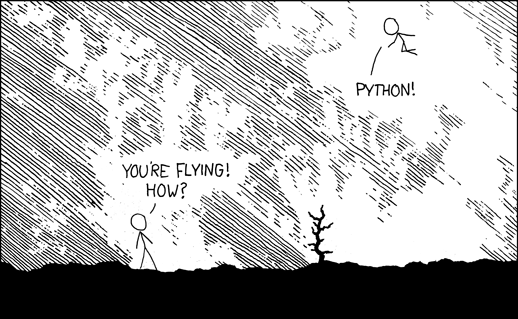
\includegraphics[height=4cm]{pics/xkcd-353.png}
    \caption{\url{http://xkcd.com/353/}}
  \end{figure}

  \small
  \begin{alertblock}{}
    \centering
    Añadido en Python 3, pero también está disponible en Python 2.7
  \end{alertblock}
\end{frame}

\begin{frame}[fragile]{6. El módulo antigravedad}
  \begin{exampleblock}{\small antigravity.py}
    \small
    \begin{lstlisting}
>>> print inspect.getsource(antigravity)
import webbrowser
webbrowser.open("http://xkcd.com/353/")
    \end{lstlisting}
  \end{exampleblock}

  \begin{center}
     \small
     En Py3K el módulo \structure{antigravity} incluye la función
     \structure{geohash()}, referencia a otra viñeta de XKCD en la que
     se describe un algoritmo que genera coodenadas en base a la fecha
     y tu posición actual: \url{http://xkcd.com/426/}
  \end{center}

  \small
  \begin{block}{\centering The History of Python - import antigravity}
    \centering
    \scriptsize
    \url{http://python-history.blogspot.com.es/2010/06/import-antigravity.html}
  \end{block}
\end{frame}

% Author: Victor Terron (c) 2014
% Email: `echo vt2rron1iaa32s | tr 132 @.e`
% License: CC BY-SA 4.0

\begin{frame}{07. \_\_str\_\_() y \_\_repr\_\_()}
  \begin{center}
    \small
    La documentación de Python hace referencia a que el método mágico
    \structure{\_\_str\_\_()} ha de devolver la representación
    ``informal'' del objeto, mientras que \structure{\_\_repr\_\_()}
    la ``formal''.
  \end{center}

  \begin{block}{}
    \centering
    \Large
    ¿Eso exactamente qué significa?
  \end{block}
\end{frame}

\begin{frame}{07. Imprimiendo un objeto Triangulo}
  \footnotesize
  \pythoncode{./code/07/700-neither-str-nor-repr.py}
  \pythonoutput{./code/07/output/700-neither-str-nor-repr}
\end{frame}

\begin{frame}{07. \_\_str\_\_()}
  \begin{block}{}
    \centering
    La función \structure{\_\_str\_\_()} debe devolver la
    \structure{cadena de texto} que se muestra por pantalla si
    llamamos a la función \structure{str()}.
  \end{block}

  \begin{center}
    \small
    Esto es lo que hace Python cuando usamos \structure{print}.
  \end{center}
\end{frame}

\begin{frame}{07. \_\_str\_\_() — Ejemplo}
  \scriptsize
  \pythoncode{./code/07/701-str-example-0.py}
  \pythonoutput{./code/07/output/701-str-example-0}
\end{frame}

\begin{frame}{07. \_\_str\_\_()}
  \begin{block}{}
    \centering
    No obstante, es mejor hacerlo sin \textit{hard-codear} el nombre
    de la clase, para que nuestro código sea más reusable.
  \end{block}

  \begin{center}
    Podemos acceder al atributo mágico \structure{\_\_name\_\_} de la
    clase actual, \structure{type(self)}, para obtener el nombre de la
    clase como una cadena de texto.
  \end{center}
\end{frame}

\begin{frame}{07. \_\_str\_\_() — Mejor así}
  \scriptsize
  \pythoncode{./code/07/702-str-example-1.py}
  \pythonoutput{./code/07/output/702-str-example-1}
\end{frame}

\begin{frame}{07. \_\_str\_\_()}
  \begin{alertblock}{}
    \Large
    \centering
    El objetivo de \structure{\_\_str\_\_()} es ser legible.
  \end{alertblock}

  \begin{center}
    La cadena que devuelve \structure{str()} no tiene otro fin que el
    de ser fácil de comprender \structure{por humanos}: cualquier cosa
    que aumente la legibilidad, como eliminar decimales inútiles o
    información poco importante, es aceptable.
  \end{center}
\end{frame}

\begin{frame}{07. \_\_repr\_\_()}
  \begin{alertblock}{}
    \large
    \centering
    El objetivo de \structure{\_\_repr\_\_()} es ser inequívoco.
  \end{alertblock}

  \begin{center}
    De \structure{\_\_repr\_\_()}, por el otro lado, se espera que nos
    devuelva una cadena de texto con una \structure{representación
    única} del objeto. Nos hace falta, por ejemplo, si estamos
    depurando un error y necesitamos saber, analizando unos logs, qué
    es exactamente uno de los objetos de la clase.
  \end{center}
\end{frame}

\begin{frame}{07. \_\_repr\_\_()}
  \begin{block}{}
    \large
    \centering
    A esta representación única se accede con la función
    \structure{repr()} o las comillas hacia atrás (\`{}\`{}).
  \end{block}

  \begin{center}
    \small
    Si \structure{\_\_repr\_\_()} no está definido, Python, en vez de
    dar un error, nos genera una representación automática, indicando
    el nombre de la clase y la dirección en memoria del objeto.
  \end{center}
\end{frame}

\begin{frame}{07. \_\_repr\_\_() — No definido}
  \footnotesize
  \pythoncode{./code/07/703-repr-undefined.py}
  \pythonoutput{./code/07/output/703-repr-undefined}
\end{frame}

\begin{frame}{07. \_\_repr\_\_()}
  \begin{alertblock}{}
    \centering
    Idealmente, la cadena devuelta por \structure{\_\_repr\_\_()}
    debería ser aquella que, pasada a \structure{eval()}, devuelve el
    mismo objeto.
  \end{alertblock}

  \begin{center}
    \small
    Al fin y al cabo, si \structure{eval()} es capaz de reconstruir el
    objeto a partir de ella, esto garantiza que contiene
    \structure{toda la infomación} necesaria.
  \end{center}
\end{frame}

\begin{frame}{07. \_\_repr\_\_() y eval()}
  \scriptsize
  \pythoncode{./code/07/704-repr-example.py}
  \pythonoutput{./code/07/output/704-repr-example}
\end{frame}

\begin{frame}{07. \_\_repr\_\_() sin  \_\_str\_\_()}
  \begin{block}{}
    \centering
    En caso de que nuestra clase defina \structure{\_\_repr\_\_()}
    pero no \structure{\_\_str\_\_()}, la llamada a \structure{str()}
    también devuelve \structure{\_\_repr\_\_()}.
  \end{block}
\end{frame}

\begin{frame}{07. \_\_repr\_\_() sin \_\_str\_\_() — Ejemplo}
  \footnotesize
  \pythoncode{./code/07/705-repr-no-str.py}
  \pythonoutput{./code/07/output/705-repr-no-str}
\end{frame}

\begin{frame}{07. \_\_repr\_\_() sin  \_\_str\_\_()}
  \begin{block}{}
    \centering
    Por eso en el primer ejemplo veíamos el nombre de la clase y su
    dirección en memoria: la llamada a \structure{\_\_str\_\_()}
    falló, por lo que Python nos devolvió \structure{\_\_repr\_\_()}.
  \end{block}

  \begin{alertblock}{}
    \small
    \centering
    El único que de verdad tenemos que implementar es
    \structure{\_\_repr\_\_()}.
  \end{alertblock}
\end{frame}

\begin{frame}{07. \_\_str\_\_() y \_\_repr\_\_() — Ejemplo}
  \footnotesize
  \pythoncode{./code/07/706-datetime-str-and-repr.py}
  \pythonoutput{./code/07/output/706-datetime-str-and-repr}
\end{frame}

\begin{frame}{07. \_\_str\_\_() y \_\_repr\_\_()}
  \small
  \begin{block}
    {\centering Difference between \_\_str\_\_ and \_\_repr\_\_ in Python}
    \centering
    \url{http://stackoverflow.com/q/1436703}
  \end{block}

  \vspace{0.5cm}
  {
    \normalsize
    \begin{alertblock}{\centering Moraleja}
      \centering
      \_\_repr\_\_() es para desarrolladores, \_\_str\_\_() para
      usuarios.
    \end{alertblock}
  }
\end{frame}

% Author: Victor Terron (c) 2013
% Email: `echo vt2rron1iaa32s | tr 132 @.e`
% License: CC BY-SA 4.0

\begin{frame}[fragile]{8. Concatenación eficiente de cadenas}
  \small
  \begin{exampleblock}
    {Tenemos varias cadenas de texto que queremos unir:}
    \small
    \begin{lstlisting}
>>> palabras = "uno", "dos", "tres"
>>> resultado = ""
>>> for p in palabras:
>>>     resultado += p
>>> resultado
'unodostres'
    \end{lstlisting}
  \end{exampleblock}

  \begin{block}{}
    Las cadenas de texto en Python son \structure{inmutables}, por lo
    que cada vez que asignamos una cadena a una variable \structure{un
    nuevo objeto} es creado en memoria. En este código estamos
    calculando, almacenando y desechando cada paso intermedio.
    Eso es inaceptablemente lento.
  \end{block}
\end{frame}

\begin{frame}[fragile]{8. Concatenación eficiente de cadenas}
  \begin{alertblock}
    {\centering \small
      La forma Pythónica de concatenar cadenas es así:}
    \centering \Large resultado = "".join(palabras)
  \end{alertblock}

  \small
  \begin{center}
    El método \structure{str.join(iterable)} devuelve una cadena que
    es la concatenación de las cadenas en \structure{iterable},
    utilizando como separador entre los elementos la cadena que llama
    al método.
  \end{center}

  \begin{exampleblock}{}
    \begin{lstlisting}
>>> palabras = "uno", "dos", "tres"
>>> "-".join(palabras)
'uno-dos-tres'
    \end{lstlisting}
  \end{exampleblock}

  \small
  \begin{center}
    Y lo hace \structure{de una única pasada} --- rápido y eficiente.
  \end{center}
\end{frame}

\begin{frame}[fragile]{9. printf en Python}
  \small
  \begin{block}{}
    \centering
    Los objetos str y unicode tienen el \structure{operador \%}, que
    nos permite usar la sintaxis del antediluviano, presente en todos
    los lenguajes, \structure{printf()}, para controlar exactamente
    cómo se muestra una cadena de texto.
  \end{block}

  \footnotesize
  \begin{exampleblock}{}
    \begin{lstlisting}
>>> print math.pi
3.14159265359
>>> "%.2f" % math.pi
3.14
>>> "%05.2f" % math.pi
03.14
>>> potencia = math.e ** 100
>>> "%.2f ^ %.2f = %.4g" % (math.e, 100, potencia)
'2.72 ^ 100.00 = 2.688e+43'
    \end{lstlisting}
  \end{exampleblock}
\end{frame}

\begin{frame}[fragile]{9. printf en Python}
  \footnotesize
  \begin{exampleblock}{}
    \begin{lstlisting}
>>> "%s por %d es %f" % ("tres", 2, 6.0)
'tres por 2 es 6.000000'
>>> "%0*d" % (5, 3)
'00003'
>>> "%+.*f" % (5, math.pi)
'+3.14159'
    \end{lstlisting}
  \end{exampleblock}

  \begin{alertblock}{}
    \centering
    \small
    No obstante, desde Python 2.6 lo recomendable es usar
    \structure{str.format()}: más sofisticado, flexible, extensible y
    que puede trabajar con tuplas y diccionarios de forma natural. ¡El
    operador de \% para el formateo de cadenas se considera
    \structure{obsoleto}!
  \end{alertblock}

  \begin{block}
    {\centering PEP 3101: Advanced String Formatting [2006]}
    \centering \url{http://www.python.org/dev/peps/pep-3101/}
  \end{block}
\end{frame}

% Author: Victor Terron (c) 2013
% Email: `echo vt2rron1iaa32s | tr 132 @.e`
% License: CC BY-SA 4.0

\begin{frame}[fragile]{10. str.format()}
  \small
  \begin{block}{}
    \centering
    Tanto el operador \structure{\%} como \structure{str.format()}
    permiten acceder a argumentos por su nombre, lo que es
    especialmente útil si necesitamos usar más de una vez la misma
    cadena. Pero \structure{str.format()} puede hacer muchas cosas
    más, como acceder a atributos de los argumentos, o hacer
    conversiones a str() y repr().
  \end{block}

  \footnotesize
  \begin{exampleblock}
    {Acceso a los argumentos por posición}
    \begin{lstlisting}
>>> '{0}{1}{0}'.format('abra', 'cad')
'abracadabra'
    \end{lstlisting}
  \end{exampleblock}

  \begin{exampleblock}
    {Acceso a los atributos de un argumento por posición}
    \begin{lstlisting}
>>> "Parte real: {0.real}".format(2+3j)
'Parte real: 2.0'
    \end{lstlisting}
  \end{exampleblock}
\end{frame}

\begin{frame}[fragile]{10. str.format()}
  \footnotesize
  \begin{exampleblock}
    {Acceso a argumentos por nombre}
    \scriptsize
    \begin{lstlisting}
>>> kwargs = {'nombre' : 'Pedro', 'apellido' : 'Medina'}
>>> "{nombre} {apellido} se llama {nombre}".format(kwargs)
'Pedro Medina se llama Pedro'
    \end{lstlisting}
  \end{exampleblock}

  \begin{exampleblock}
    {Acceso a atributos de argumentos por nombre}
    \scriptsize
    \begin{lstlisting}
>>> kwargs = {'numero' : 1+5j}
>>> "Parte imaginaria: {numero.imag}".format(**kwargs)
'Parte imaginaria: 5.0'
    \end{lstlisting}
  \end{exampleblock}

  \small
  \begin{block}
    {\centering Format Specification Mini-Language}
    \footnotesize
    \centering
    \url{http://docs.python.org/2/library/string.html#formatstrings}
  \end{block}
\end{frame}


\section{Los diez siguientes}

% Author: Victor Terron (c) 2013
% Email: `echo vt2rron1iaa32s | tr 132 @.e`
% License: CC BY-SA 4.0

\begin{frame}[fragile]{11. Cadenas multilínea}

  \begin{block}{}
    \centering \large
    Una opción es usar \structure{barras invertidas}
  \end{block}

  \begin{exampleblock}{}
    \scriptsize
    \begin{lstlisting}
>>> parrafo = "En un lugar de la Mancha, de cuyo nombre " \
...           "no quiero acordarme, no ha mucho tiempo " \
...           "que vivía un hidalgo de los de lanza en " \
...           "astillero, adarga antigua, rocín flaco y " \
...           "galgo corredor."
>>> parrafo[:24]
'En un lugar de la Mancha'
>>> parrafo[-17:]
'y galgo corredor.'
    \end{lstlisting}
  \end{exampleblock}

  \begin{alertblock}{}
    \centering
    \small
    Pero, en el caso de trabajar con \structure{cadenas muy largas},
    puede ser molesto tener que \structure{terminar cada línea con
      \textbackslash}, sobre todo porque nos impide reformatear el
    párrafo con nuestro entorno de desarrollo o editor de texto ---
    ¡Emacs, por supuesto!
  \end{alertblock}
\end{frame}

\begin{frame}[fragile]{11. Cadenas multilínea}

  \begin{block}{}
    \centering
    Las comillas triples respetan \structure{todo} lo que hay dentro
    de ellas, incluyendo \structure{saltos de línea}. No es necesario
    escapar nada: todo se incluye directamente en la cadena.
  \end{block}

  \begin{exampleblock}{}
    \scriptsize
    %Escape triple quotes; otherwise string is italicized
    \begin{lstlisting}[escapechar=!]
>>> parrafo = !"""!En un lugar de la Mancha,
... de cuyo nombre no quiero
... acordarme
...
... !"""!
>>> print parrafo
En un lugar de la Mancha,
de cuyo nombre no quiero
acordarme


>>>
    \end{lstlisting}
  \end{exampleblock}
\end{frame}

\begin{frame}[fragile]{11. Cadenas multilínea}

  \begin{alertblock}{}
    \small
    \centering
    Una opción menos conocida es que podemos dividir nuestra cadena en
    líneas, una por línea, y \structure{rodearlas con paréntesis}.
    Python evalúa lo que hay dentro de los mismos y de forma
    automática las concatena:
   \end{alertblock}

  \begin{exampleblock}{}
    \scriptsize
    \begin{lstlisting}
>>> parrafo =  ("Es, pues, de saber, que este "
...             "sobredicho hidalgo, los ratos "
...             "que estaba ocioso")
>>> len(parrafo.split())
13
    \end{lstlisting}
  \end{exampleblock}

  \small
  \begin{exampleblock}
    {Un ejemplo más sencillo:}
    \begin{lstlisting}
>>> "uno" "dos"
'unodos'
    \end{lstlisting}
  \end{exampleblock}
\end{frame}

% Author: Victor Terron (c) 2013
% Email: `echo vt2rron1iaa32s | tr 132 @.e`
% License: CC BY-SA 4.0

\begin{frame}[fragile]
  {\large 12. Listas por comprensión vs generadores}
  \begin{block}{}
    \small
    \centering
    Las listas por comprensión nos permiten construir, \structure{en
    un único paso}, una lista donde cada elemento es el resultado de
    aplicar \structure{algunas operaciones} a todos (o algunos de) los
    miembros de otra secuencia o iterable.
  \end{block}

  \footnotesize
  \begin{exampleblock}
    {Por ejemplo, para calcular el cuadrado de los números [0, 9]:}
    \begin{lstlisting}
>>> g = [x ** 2 for x in range(10)]
[0, 1, 4, 9, 16, 25, 36, 49, 64, 81]
    \end{lstlisting}
  \end{exampleblock}

  \begin{exampleblock}
    {Esto es equivalente a:}
    \begin{lstlisting}
>>> resultado = []
>>> for x in range(10):
...     resultado.append(x ** 2)
    \end{lstlisting}
  \end{exampleblock}
\end{frame}

\begin{frame}[fragile]
  {\large 12. Listas por comprensión vs generadores}

  \begin{alertblock}{}
    \centering
    El problema, a veces, es que las listas por comprensión
    construyen... pues eso, una lista, almacenando \structure{todos
    los valores en memoria} a la vez.
  \end{alertblock}

  \footnotesize
  \begin{exampleblock}
    {No intentéis esto en casa}
    \begin{lstlisting}
>>> [x ** 2 for x in xrange(1000000000000000)]
# Tu ordenador explota
    \end{lstlisting}
  \end{exampleblock}
\end{frame}

\begin{frame}[fragile]
  {\large 12. Listas por comprensión vs generadores}
  \small
  \begin{block}{}
    \centering
    Si sólo necesitamos los valores una vez, y de uno en uno, podemos
    utilizar una \structure{expresión generadora}: son idénticos a las
    listas por comprensión, pero usando \structure{paréntesis}.
  \end{block}

  \footnotesize
  \begin{exampleblock}{}
    \begin{lstlisting}
>>> cuadrados = (x ** 2 for x in range(1, 11))
>>> cuadrados
<generator object <genexpr> at 0x7f8b82504eb0>
>>> next(cuadrados)
1
>>> next(cuadrados)
4
    \end{lstlisting}
  \end{exampleblock}

  \small
  \begin{block}
    {\centering PEP 289: Generator Expressions}
    \centering \url{http://www.python.org/dev/peps/pep-0289/}
  \end{block}
\end{frame}

\begin{frame}[fragile]
  {\large 12. Listas por comprensión vs generadores}
  \footnotesize
  \begin{exampleblock}
    {Equivalente a:}
    \begin{lstlisting}
>>> def cuadrados(seq):
...     for x in seq:
...         yield x ** 2
...
>>> g = cuadrados(range(1, 11))
>>> next(g)
1
>>> next(g)
4
    \end{lstlisting}
  \end{exampleblock}

  \small
  \begin{block}
    {\centering Generator Tricks for Systems Programmers (David M. Beazley)}
    \centering \url{http://www.dabeaz.com/generators/}
  \end{block}
\end{frame}

% Author: Victor Terron (c) 2013
% Email: `echo vt2rron1iaa32s | tr 132 @.e`
% License: CC BY-SA 4.0

\begin{frame}[fragile]{13. \large Comprensión de conjuntos y diccionarios}
  \begin{block}{}
  \centering
    En Python 2.7.x+ y 3.x+ podemos crear no sólo listas, sino también
    \structure{conjuntos} y \structure{diccionarios} por comprensión.
  \end{block}

  \scriptsize
  \begin{exampleblock}
    {Un conjunto con los múltiplos de siete <= 100:}
    \begin{lstlisting}
>>> {x for x in range(1, 101) if not x % 7}
set([98, 35, 70, 7, 42, 77, 14, 49, 84, 21, 56, 91, 28, 63])
    \end{lstlisting}
  \end{exampleblock}

  \begin{exampleblock}
    {Otra forma de hacerlo:}
    \begin{lstlisting}
>>> mult7 = set(x for x in range(1, 101) if not x % 7)
>>> len(mult7)
14
>>> 25 in mult7
False
    \end{lstlisting}
  \end{exampleblock}
\end{frame}

\begin{frame}[fragile]{13. \large Comprensión de conjuntos y diccionarios}
  \scriptsize
  \begin{exampleblock}
    {Un diccionario con el cubo de los números [0, 9]:}
    \begin{lstlisting}
>>> cubos = {x : x ** 3 for x in range(10)}
>>> cubos[2]
8
>>> cubos[8]
512
    \end{lstlisting}
  \end{exampleblock}

  \begin{exampleblock}
    {Otra forma de hacerlo:}
    \begin{lstlisting}
>>> dict((x, x ** 3) for x in range(5))
{0: 0, 1: 1, 2: 8, 3: 27, 4: 64}
    \end{lstlisting}
  \end{exampleblock}

  \small
  \begin{block}
    {\centering PEP 274: Dict Comprehensions [2001]}
    \centering \url{http://www.python.org/dev/peps/pep-0274/}
  \end{block}
\end{frame}

\begin{frame}[fragile]
  {14. \normalsize Repeticiones innecesarias en 'if' compuestos}
  \small
  \begin{block}{}
    \centering
    A veces podemos \structure{simplificar} algunas expresiones
    lógicas. Por ejemplo, si tenemos una serie de valores y queremos
    comprobar si nuestra variable es \structure{igual a alguno de
    ellos}:
  \end{block}

  \footnotesize
  \begin{exampleblock}
    {No escribas esto:}
    \begin{lstlisting}
>> x = 4
>> x == 3 or x == 5 or x == 7:
False
    \end{lstlisting}
  \end{exampleblock}

  \begin{exampleblock}
    {Mejor hacerlo así:}
    \begin{lstlisting}
>> x in (3, 5, 7)
False
    \end{lstlisting}
  \end{exampleblock}
\end{frame}

\begin{frame}[fragile]
  {14. \normalsize Repeticiones innecesarias en 'if' compuestos}
  \begin{block}{}
    \centering
    \structure{any()} devuelve \structure{True} si al menos un
    elemento del iterable que recibe evalúa a verdadero. También
    devuelve \structure{False} si el iterable está vacío.
  \end{block}

  \begin{exampleblock}{}
    \begin{lstlisting}
>>> any([False, True, False])
True
>>> any([False, False])
False
>>> any([])
False
    \end{lstlisting}
  \end{exampleblock}
\end{frame}

\begin{frame}[fragile]
  {14. \normalsize Repeticiones innecesarias en 'if' compuestos}
  \footnotesize
  \begin{exampleblock}
    {¿Hay algún número par?}
    \begin{lstlisting}
>>> numeros = [3, 7, 8, 9]
>>> any([not x % 2 for x in numeros])
True
    \end{lstlisting}
  \end{exampleblock}

  \normalsize
  \begin{alertblock}{}
    \centering
    Aún mejor: podemos usar un \structure{generador}
  \end{alertblock}

  \footnotesize
  \begin{exampleblock}{}
    \begin{lstlisting}[escapechar=!]
>>> numeros = [3, 7, 9, 11]
>>> any!\color{red}{(}!not x % 2 for x in numeros!\color{red}{)}!
False
    \end{lstlisting}
  \end{exampleblock}

  \small
  \begin{block}
    {\centering Built-in Functions: any()}
    \centering \url{http://docs.python.org/2/library/functions.html\#any}
  \end{block}
\end{frame}

\begin{frame}[fragile]
  {14. \normalsize Repeticiones innecesarias en 'if' compuestos}
  \begin{block}{}
    \centering
    \structure{all()} devueve True si \structure{todos} los elementos
    del iterable evalúan a verdadero, o si éste está vacío.
  \end{block}

  \begin{exampleblock}{}
    \begin{lstlisting}
>>> all([False, True, False])
False
>>> all([True])
True
>>> all([])
True
    \end{lstlisting}
  \end{exampleblock}
\end{frame}

\begin{frame}[fragile]
  {14. \normalsize Repeticiones innecesarias en 'if' compuestos}
  \begin{exampleblock}
    {¿Son pares todos los números?}
    \begin{lstlisting}
>>> numeros = [1, 4, 6, 8]
>>> all(not x % 2 for x in numeros)
False
    \end{lstlisting}
  \end{exampleblock}
\end{frame}

\begin{frame}[fragile]
  {14. \normalsize Repeticiones innecesarias en 'if' compuestos}
  \begin{alertblock}{}
    \centering
    Infinitamente mejor que la alternativa de, quizás:
  \end{alertblock}

  \footnotesize
  \begin{exampleblock}{}
    \begin{lstlisting}
>>> numeros = [1, 4, 6, 8]
>>> son_pares = True
>>> for x in numeros:
...     if x % 2:
...         son_pares = False
...         break
...
>>> son_pares
False
    \end{lstlisting}
  \end{exampleblock}

  \small
  \begin{block}
    {\centering Built-in Functions: all()}
    \centering \url{http://docs.python.org/2/library/functions.html\#all}
  \end{block}
\end{frame}

\begin{frame}[fragile]{15. pow(x, y, z)}
  \small
  \begin{block}{}
    \centering
    La función \structure{pow()} acepta, opcionalmente, un tercer
    argumento, \structure{z}. En caso de especificarse, la función
    devuelve \structure{pow(x, y) \% z}.  No es sólo práctico en
    algunos escenarios, sino que su implementación es más rápida que
    calcularlo nosotros en dos pasos.
  \end{block}

  \footnotesize
  \begin{exampleblock}{}
    \begin{lstlisting}
>>> pow(2, 3)
8
>>> pow(2, 3, 6)
2
>>> pow(2, 5, 17)
15
    \end{lstlisting}
  \end{exampleblock}

  \small
  \begin{block}
    {\centering Built-in Functions: pow()}
    \centering \url{http://docs.python.org/2/library/functions.html\#pow}
  \end{block}
\end{frame}

% Author: Victor Terron (c) 2013
% Email: `echo vt2rron1iaa32s | tr 132 @.e`
% License: CC BY-SA 4.0

\begin{frame}[fragile]{16. sorted() - parámetro 'key'}
  \footnotesize
  \begin{block}{}
    \centering
    Desde Python 2.4, tanto el método \structure{list.sort()} como la
    función \structure{sorted()} aceptan el parámetro \structure{key},
    con el que se especifica la función que se ejecuta para cada
    elemento y a partir de cuyo resultado se ordena la secuencia.
  \end{block}

  \begin{exampleblock}
    {Ordenar una serie de números por su valor absoluto:}
    \begin{lstlisting}
>>> nums = [-8, 3, 5, -1, 3]
>>> sorted(nums, key=abs)
[-1, 3, 3, 5, -8]
    \end{lstlisting}
  \end{exampleblock}

  \begin{exampleblock}
    {Una lista de cadenas lexicográficamente:}
    \begin{lstlisting}
>>> gnu = ["GNU", "is", "Not", "Unix"]
>>> sorted(gnu)
['GNU', 'Not', 'Unix', 'is']
    \end{lstlisting}
  \end{exampleblock}
\end{frame}

\begin{frame}[fragile]{16. sorted() - parámetro 'key'}
  \begin{exampleblock}
    {Ahora por su longitud:}
    \begin{lstlisting}
>>> sorted(gnu, key=len)
['is', 'GNU', 'Not', 'Unix']
    \end{lstlisting}
  \end{exampleblock}

  \begin{alertblock}{}
    \centering
    Desde 2.2, las ordenaciones en Python son \structure{estables}: al
    tener 'GNU' y 'Not' la misma longitud, se mantiene el orden
    original. Esto permite ordenar en función de \structure{dos o más
    criterios}, en diferentes pasos.
  \end{alertblock}
\end{frame}

\begin{frame}[fragile]{16. sorted() - parámetro 'key'}
  \begin{block}{}
    \centering
    Podemos ordenar \structure{usando nuestras propias funciones}
  \end{block}

  \footnotesize
  \begin{exampleblock}
    {Ordenar por el número de vocales:}
    \begin{lstlisting}
>>> def nvocales(palabra):
...    contador = 0
...    for letra in palabra:
...        if letra.lower() in "aeiou":
...	   contador += 1
...    return contador
...
>>> lame = "LAME Ain't an MP3 Encoder".split()
>>> sorted(lame, key=nvocales)
['MP3', 'an', 'LAME', "Ain't", 'Encoder']
    \end{lstlisting}
  \end{exampleblock}
\end{frame}

\begin{frame}[fragile]{16. sorted() - parámetro 'key'}
  \begin{block}{}
    \centering
    O usando \structure{funciones anónimas}
  \end{block}

  \footnotesize
  \begin{exampleblock}
    {Ordenar por la parte compeja:}
    \begin{lstlisting}
>>> nums = [7+9j, 4-5j, 3+2j]
>>> sorted(nums, key=lambda x: x.imag)
[(4-5j), (3+2j), (7+9j)]
    \end{lstlisting}
  \end{exampleblock}

  \begin{exampleblock}
    {Ordenar por el segundo elemento de la tupla:}
    \begin{lstlisting}
>>> puntos = [(2, 3), (5, 1), (3, 4), (8, 2)]
>>> sorted(puntos, key=lambda x: x[1])
[(5, 1), (8, 2), (2, 3), (3, 4)]
    \end{lstlisting}
  \end{exampleblock}

  \begin{block}
    {\centering Sorting Mini-HOW TO}
    \centering \url{http://wiki.python.org/moin/HowTo/Sorting/}
  \end{block}
\end{frame}

% Author: Victor Terron (c) 2013
% Email: `echo vt2rron1iaa32s | tr 132 @.e`
% License: CC BY-SA 4.0

\begin{frame}[fragile]{17. Por qué "python" > [130, 129]}
  \small
  \begin{block}{}
    \centering
    Listas y tuplas se ordenan \structure{lexicográficamente},
    comparando uno a uno los elementos. Para ser iguales, ambas
    secuencias han de tener el mismo \structure{tipo}, la misma
    \structure{longitud} y sus elementos ser \structure{iguales}.
  \end{block}

  \begin{exampleblock}{}
    \begin{lstlisting}
>>> [1, 2] == [1, 2]
True
>>> [1, 2] == [3, 4]
False
>>> [1, 2] == (1, 2)
False
    \end{lstlisting}
  \end{exampleblock}
\end{frame}

\begin{frame}[fragile]{17. Por qué "python" > [130, 129]}
  \small
  \begin{alertblock}{}
    \centering
    En caso de \structure{no} tener el mismo número de elementos, la
    comparación de las dos secuencias está determinada por el primer
    elemento en el que sus valores diferen.
  \end{alertblock}

  \begin{exampleblock}{}
    \begin{lstlisting}
>>> (4, 2, 5) > (1, 3, 2)
True
>>> [2, 3, 1] >= [2, 4, 2]
False
    \end{lstlisting}
  \end{exampleblock}
\end{frame}

\begin{frame}[fragile]{17. Por qué "python" > [130, 129]}
  \small
  \begin{block}{}
    \centering
    Si el elemento correspondiente, donde los valores difieren, no
    existe, \structure{la secuencia más corta} va antes.
  \end{block}

  \begin{exampleblock}{}
    \begin{lstlisting}
>>> (2, 3) > (1,2,3)
True
>>> [1, 2] < [1, 2, 3]
True
    \end{lstlisting}
  \end{exampleblock}
\end{frame}

\begin{frame}[fragile]{17. Por qué "python" > [130, 129]}
  \small
  \begin{alertblock}{}
    \centering
    Los objetos de tipos diferentes nunca se consideran iguales, y se
    ordenan de forma \structure{consistente pero arbitraria}. En
    CPython, el criterio escogido es el del nombre de sus tipos.
  \end{alertblock}

  \footnotesize
  \begin{exampleblock}{}
    \begin{lstlisting}[escapechar=!]
>>> "python" > [130, 129]    # "str" > "list"
True
>>> {1 : "uno"} > [1, 2, 3]  # "dict" < "list"
False
>>> (23,) > [34, 1]          # "tuple" > "list"
True
    \end{lstlisting}
  \end{exampleblock}

  \begin{block}
    {\centering Stack Overflow: Maximum of two tuples}
    \centering \url{http://stackoverflow.com/a/9576006/184363}
  \end{block}
\end{frame}

\begin{frame}[fragile]{17. Por qué "python" > [130, 129]}
  \begin{block}{}
    \centering
    Pero un tipo de dato \structure{numérico} va siempre antes si lo
    comparamos con uno \structure{no numérico}.
  \end{block}

  \footnotesize
  \begin{exampleblock}{}
    \begin{lstlisting}
>>> 23 < "Python"
True
>>> 23 < (3, 1, 4)
True
>>> 23 > [3, 1, 4]
False
>>> 23 < {"pi" : 3.1415}
True
    \end{lstlisting}
  \end{exampleblock}

  \begin{block}
    {\centering Stack Overflow: How does Python compare string and int?}
    \centering \url{http://stackoverflow.com/a/3270689/184363}
  \end{block}
\end{frame}

\begin{frame}[fragile]{17. Por qué "python" > [130, 129]}
  \begin{alertblock}{}
    \centering
    Esto es un detalle de la \structure{implementación} de
    \structure{CPython}.
  \end{alertblock}

  \small
  \begin{center}
    Nuestro código nunca debería depender de que valores de diferente
    tipos se ordenen así. Y, en cualquier caso, ¿qué haces comparando
    valores de diferente tipo? ¿Por qué querrías hacer eso?
  \end{center}

  \begin{exampleblock}
    {\centering En Py3K el comportamiento ya es el que esperaríamos:}
    \begin{lstlisting}
>>> 23 < "Python"
Traceback (most recent call last):
  File "<stdin>", line 1, in <module>
TypeError: unorderable types: int() < str()
    \end{lstlisting}
  \end{exampleblock}
\end{frame}

% Author: Victor Terron (c) 2013
% Email: `echo vt2rron1iaa32s | tr 132 @.e`
% License: CC BY-SA 4.0

\begin{frame}[fragile]{18. Aplanando una lista con sum()}
  \begin{block}{}
    \centering \LARGE sum(iterable[, start])
  \end{block}

  \small
  \begin{center}
    \centering
    La función sum() acepta, opcionalmente, un segundo argumento,
    \structure{start}, cuyo valor por defecto es cero, al cual se van
    sumando los elementos de \structure{iterable}.
  \end{center}

  \footnotesize
  \begin{exampleblock}{}
    \begin{lstlisting}
>>> sum([1, 2, 3])
6
>>> sum([1, 2, 3], 10)
16
>>> sum(range(1, 10))
45
>>> sum([100], -1)
99
    \end{lstlisting}
  \end{exampleblock}
\end{frame}

\begin{frame}[fragile]{18. Aplanando una lista con sum()}
  \begin{block}{}
    \centering
    Podemos usar una lista vacía, [], como \structure{start}, para aplanar
    una lista de listas. La función sum(), al 'sumarlas', lo que hará será
    \structure{concatenarlas} una detrás de otra.
  \end{block}

  \small
  \begin{exampleblock}{}
    \begin{lstlisting}
>>> sum([[1, 2], [3], [4, 5], [6, 7, 8]], [])
[1, 2, 3, 4, 5, 6, 7, 8]
>>> sum([[4, 5], [6, 7]], range(4))
[0, 1, 2, 3, 4, 5, 6, 7]
    \end{lstlisting}
  \end{exampleblock}
\end{frame}

\begin{frame}[fragile]{18. Aplanando una lista con sum()}
  \begin{alertblock}{}
    \centering
    Es importante que \structure{start} sea una lista. De lo contrario,
    sum() intentará añadir cada una de las sublistas a un entero, cero.
    Y eso no se puede hacer.
  \end{alertblock}

  \scriptsize
  \begin{exampleblock}{}
    \begin{lstlisting}
>>> sum([[4, 5], [6, 7]])
Traceback (most recent call last):
  File "<stdin>", line 1, in <module>
TypeError: unsupported operand type(s) for +: 'int' and 'list'
    \end{lstlisting}
  \end{exampleblock}

  \small
  \begin{block}
    {\centering Stack Overflow - Flattening a list with sum():}
    \centering \url{http://stackoverflow.com/a/6632253/184363 }
  \end{block}
\end{frame}

% Author: Victor Terron (c) 2013
% Email: `echo vt2rron1iaa32s | tr 132 @.e`
% License: CC BY-SA 4.0

\begin{frame}[fragile]{19. El operador ternario}
  \begin{center}
    El operator ternario (o condicional) nos permite escoger entre dos
    expresiones en \structure{función de una tercera}, la condición.
  \end{center}

  \begin{block}
    {\small
      En casi todos los lenguajes de programación tiene la misma forma:}
    \centering \LARGE test ? a : b
  \end{block}

  \begin{exampleblock}{Por ejemplo, en C:}
    \begin{lstlisting}[language=C]
int nsecs = (counter > 5) ? 5 : 0;
    \end{lstlisting}
  \end{exampleblock}
\end{frame}

\begin{frame}[fragile]{19. El operador ternario}
  \begin{center}
    En Python se conocen como \structure{expresiones condicionales}, y
    existen desde la versión 2.5. Su sintaxis es:
  \end{center}

  \begin{block}{}
    \centering \LARGE a if test else b
  \end{block}

  \begin{exampleblock}{}
    \begin{lstlisting}
>>> x = 2
>>> "uno" if x == 1 else "otra cosa"
'otra cosa'
    \end{lstlisting}
  \end{exampleblock}
\end{frame}

\begin{frame}[fragile]{19. El operador ternario}
  \footnotesize
  \begin{exampleblock}{}
    \begin{lstlisting}
>>> hora = 17
>>> msg = ("Es la" if hora == 1 else "Son las")
>>> msg + " {0}h".format(hora)
'Son las 17h'
    \end{lstlisting}
  \end{exampleblock}

  \begin{exampleblock}
    {Eleva al cuadrado si x es impar, divide entre dos de lo contrario:}
    \begin{lstlisting}
>>> x = 13
>>> y = x ** 2 if x % 2 else x / 2
>>> y
169
    \end{lstlisting}
  \end{exampleblock}

  \small
  \begin{block}
    {\centering PEP 308: Conditional Expressions [2003]}
    \centering \url{http://www.python.org/dev/peps/pep-0308/}
  \end{block}
\end{frame}

% Author: Victor Terron (c) 2013
% Email: `echo vt2rron1iaa32s | tr 132 @.e`
% License: CC BY-SA 4.0

\begin{frame}[fragile]
  {20. \large Incremento != 1 en el operador slice}
  \begin{block}{}
    \centering \LARGE x[start:end:step]
  \end{block}

  \small
  \begin{center}
    El tercer índice, opcional, del \structure{operador slice},
    especifica el tamaño del paso --- cuánto avanzamos cada vez.
    Por defecto es uno, y por eso:
  \end{center}

  \begin{exampleblock}
    {Los tres primeros elementos}
    \begin{lstlisting}
>>> x = range(1, 10)
>>> x[:3]
[0, 1, 2]
    \end{lstlisting}
  \end{exampleblock}
\end{frame}

\begin{frame}[fragile]
  {20. \large Incremento != 1 en el operador slice}
  \begin{exampleblock}
    {Los cuatro últimos}
    \begin{lstlisting}
>>> x[-4:]
[6, 7, 8, 9]
    \end{lstlisting}
  \end{exampleblock}

  \begin{exampleblock}
    {Del segundo al quinto}
    \begin{lstlisting}
>>> x[1:5]
[1, 2, 3, 4]
    \end{lstlisting}
  \end{exampleblock}
\end{frame}

\begin{frame}[fragile]
  {20. \large Incremento != 1 en el operador slice}
  \begin{block}{}
    \large
    \centering
    Podemos usar un paso \structure{distinto de uno}
  \end{block}

  \small
  \begin{exampleblock}
    {Elementos en posiciones pares...}
    \begin{lstlisting}
>>> x[::2]
[1, 3, 5, 7, 9]
    \end{lstlisting}
  \end{exampleblock}

  \begin{exampleblock}
    {... e impares}
    \begin{lstlisting}
>>> x[1::2]
[0, 2, 4, 6, 8]
    \end{lstlisting}
  \end{exampleblock}
\end{frame}

\begin{frame}[fragile]
  {20. \large Incremento != 1 en el operador slice}
  \begin{exampleblock}
    {Recorrer los primeros nueve elementos, de tres en tres}
    \begin{lstlisting}
>>> x[:9:3]
[0, 3, 6]
    \end{lstlisting}
  \end{exampleblock}

  \begin{alertblock}{}
    \small
    \centering
    Hacia adelante, empezamos a contar en \structure{cero}, terminamos
    en \structure{n-1}
  \end{alertblock}
\end{frame}

\begin{frame}[fragile]
  {20. \large Incremento != 1 en el operador slice}
  \begin{block}{}
    \centering
    Un paso negativo permite recorrer la lista \structure{hacia atrás}
  \end{block}

  \small
  \begin{exampleblock}
    {Invierte la lista}
    \begin{lstlisting}
>>> x[::-1]
[9, 8, 7, 6, 5, 4, 3, 2, 1, 0]
    \end{lstlisting}
  \end{exampleblock}

  \begin{exampleblock}
    {Recorre la lista hacia atrás, de dos en dos}
    \begin{lstlisting}
>>> x[::-2]
[9, 7, 5, 3, 1]
    \end{lstlisting}
  \end{exampleblock}
\end{frame}

\begin{frame}[fragile]
  {20. \large Incremento != 1 en el operador slice}
  \begin{exampleblock}
    {Del último hasta el tercero, no inclusive, hacia atrás}
    \begin{lstlisting}
>>> x[:2:-1]
[9, 8, 7, 6, 5, 4, 3]
    \end{lstlisting}
  \end{exampleblock}

  \begin{alertblock}{}
    \small
    \centering
    Hacia atrás, empezamos a contar en \structure{-1}, terminamos
    en \structure{-len}
  \end{alertblock}
\end{frame}


\section{}

\begin{frame}{}
  \begin{block}{}
    \centering \Large Respira profundamente
  \end{block}

  \begin{figure}
    \centering
    
\includegraphics[height=6cm]{pics/a-clockwork-orange-2.jpg}
  \end{figure}
\end{frame}

\section{Diez más}

% Author: Victor Terron (c) 2013
% Email: `echo vt2rron1iaa32s | tr 132 @.e`
% License: CC BY-SA 4.0

\begin{frame}[fragile]{21. La variable \_}
  \begin{alertblock}{}
    \small
    \centering
    En el modo interactivo (Python shell), la variable \structure{\_}
    siempre contiene el valor del \structure{último} \emph{statement}
    ejecutado. Es muy útil si necesitamos \structure{reusar} el último
    valor que hemos calculado y olvidamos almacenarlo en una variable:
  \end{alertblock}

  \footnotesize
  \begin{exampleblock}{}
    \begin{lstlisting}
>>> 3 * 4
12
>>> _ + 1
13
>>> _ ** 2
169
>>> range(10)
[0, 1, 2, 3, 4, 5, 6, 7, 8, 9]
>>> _[-1]
9
    \end{lstlisting}
  \end{exampleblock}
\end{frame}

\begin{frame}[fragile]{21. La variable \_}
  \begin{block}{}
    \small
    \centering
    En modo no-interactivo (un script en Python cualquiera),
    \structure{\_} es un nombre más de variable. Por convención, suele
    usarse como nombre de variable para indicar que es
    \structure{desechable} (\emph{throwaway variable}), cuando
    necesitamos una pero \structure{no llegamos a usarla}.
  \end{block}

  \footnotesize
  \begin{exampleblock}{}
    \begin{lstlisting}
>>> for _ in range(10):
...     print "¡Hola, mundo!"
    \end{lstlisting}
  \end{exampleblock}


  \begin{exampleblock}{}
    \begin{lstlisting}
>>> import os.path
>>> path = "curriculum.tex"
>>> _, ext = os.path.splitext(path)
>>> ext
'.tex'
    \end{lstlisting}
  \end{exampleblock}
\end{frame}

% Author: Victor Terron (c) 2013
% Email: `echo vt2rron1iaa32s | tr 132 @.e`
% License: CC BY-SA 4.0

\begin{frame}[fragile]{22. \large Funciones lambda, y qué opina GvR}
  \small
  \begin{center}
    Antes hemos usado \structure{funciones lambda} (o anónimas) para
    definir sobre la marcha funciones sencillas que sólo necesitábamos
    una vez. Recordemos:
  \end{center}

  \footnotesize
  \begin{exampleblock}
    {Ordenar por la parte compleja:}
    \begin{lstlisting}
>>> nums = [7+9j, 4-5j, 3+2j]
>>> sorted(nums, key=lambda x: x.imag)
[(4-5j), (3+2j), (7+9j)]
    \end{lstlisting}
  \end{exampleblock}

  \small
  \begin{block}{}
    \centering
    Las funciones lambda son muy útiles y cómodas en algunas
    ocasiones.  Provienen del mundo de la \structure{programación
    funcional}, al igual que las funciones de orden superior
    \structure{map()}, \structure{filter()} y \structure{reduce()}.
  \end{block}
\end{frame}

\begin{frame}[fragile]{22. \large Funciones lambda, y qué opina GvR}
  \begin{alertblock}{}
    \large
    \centering
    Pero a Guido van Rossum no le gustan.
  \end{alertblock}

  \small
  \begin{center}
    Nunca le convencieron y, de hecho, estuvieron a punto de desaparecer en Py3K.
  \end{center}

  \footnotesize
  \begin{center}
    El nombre de lambda puede dar lugar a confusión, ya que su
    semántica \structure{no es la misma} que en otros lenguajes. La
    idea de \structure{lambda} era sólo la de servir de herramienta
    sintática para definir funciones anónimas. El problema es que
    nadie ha sido capaz todavía de encontrar una forma mejor forma
    esto, por lo que \structure{lambda} sigue entre nosotros.
   \end{center}

  \begin{block}
    {\centering Origins of Python's "Functional" Features:}
    \centering \url{http://python-history.blogspot.com.es/2009/04/origins-of-pythons-functional-features.html}
  \end{block}
\end{frame}

\begin{frame}[fragile]{22. \large Funciones lambda, y qué opina GvR}
  \small
  \begin{block}{}
    \centering
    Así que \structure{lambda} sigue existiendo, pero lo Pythónico es
    usar el módulo \structure{operator}.  Más legible, más claro, más
    explícito.
  \end{block}

  \footnotesize
  \begin{exampleblock}
    {Ordenando de nuevo por la parte compleja...}
    \begin{lstlisting}
>>> import operator
>>> nums = [7+9j, 4-5j, 3+2j]
>>> sorted(nums, key=operator.attrgetter('imag'))
[(4-5j), (3+2j), (7+9j)]
    \end{lstlisting}
  \end{exampleblock}

  \begin{exampleblock}
    {... y por el segundo elemento de la tupla:}
    \begin{lstlisting}
>>> import operator
>>> puntos = [(2, 3), (5, 1), (3, 4), (8, 2)]
>>> sorted(puntos, key=operator.itemgetter(1))
[(5, 1), (8, 2), (2, 3), (3, 4)]
    \end{lstlisting}
  \end{exampleblock}
\end{frame}

% Author: Victor Terron (c) 2013
% Email: `echo vt2rron1iaa32s | tr 132 @.e`
% License: CC BY-SA 4.0

\begin{frame}[fragile]{23. Parámetros por defecto mutables}
  \begin{exampleblock}{}
    \small
    \begin{lstlisting}
>>> def inserta_uno(valores=[]):
...     valores.append(1)
...     return valores
...
>>> inserta_uno(range(3))
[0, 1, 2, 1]
>>> inserta_uno()
[1]
>>> inserta_uno()
[1, 1]
>>> inserta_uno()
[1, 1, 1]
    \end{lstlisting}
  \end{exampleblock}
\end{frame}

\begin{frame}[fragile]{23. Parámetros por defecto mutables}
  \begin{figure}
    \centering
    
\includegraphics[height=6cm]{pics/omg-face.jpg}
  \end{figure}
\end{frame}

\begin{frame}[fragile]{23. Parámetros por defecto mutables}
  \begin{block}{}
    \centering
    \small
    El motivo por el que esto ocurre es que las funciones en Python
    son objetos de primera clase, no sólo un trozo más de código:
    \structure{se evalúan cuando son definidas}, incluyendo parámetros
    por defecto, y por tanto su estado puede cambiar de una vez a
    otra.
  \end{block}

  \begin{alertblock}{}
    \centering
    Es decir, que los parámetros por defecto se evalúan sólo
    \structure{una} vez, en el momento en el que \structure{la función
    se define}.
  \end{alertblock}
\end{frame}

\begin{frame}[fragile]{23. Parámetros por defecto mutables}
  \begin{block}{}
    \centering
    La solución es usar un \structure{parámetro de sustitución}, en
    lugar de modificar directamente el valor por defecto.
  \end{block}

  \begin{exampleblock}{}
    \footnotesize
    \begin{lstlisting}
>>> def inserta_uno(valores=None):
...     if valores is None:
...         valores = []
...     valores.append(1)
...     return valores
...
>>> inserta_uno()
[1]
>>> inserta_uno()
[1]
>>> inserta_uno()
[1]
    \end{lstlisting}
  \end{exampleblock}
\end{frame}

\begin{frame}[fragile]{23. Parámetros por defecto mutables}
  \begin{alertblock}
    \large
    \centering
    ¿Y entonces esto?
  \end{alertblock}

  \begin{exampleblock}{}
    \small
    \begin{lstlisting}
>>> def suma(numeros, inicio=0):
...     for x in numeros:
...         inicio += x
...     return inicio
...
>>> suma([1, 2])
3
>>> suma([3, 4])
7
>>> suma([1, 2, 3])
6
    \end{lstlisting}
  \end{exampleblock}
\end{frame}

\begin{frame}[fragile]{23. Parámetros por defecto mutables}
  \begin{block}{}
    \centering
    La razón es que, a diferencia de las listas, los enteros en Python
    son \structure{inmutables}, por lo que no pueden modificarse de
    una llamada a otra. Por tanto, \structure{inicio} siempre es cero
    cuando llamamos a la función.
  \end{block}

  \small
  \begin{block}
    {\centering Call By Object}
    \centering \url{http://effbot.org/zone/call-by-object.htm}
  \end{block}

  \begin{block}
    {\centering Default Parameter Values in Python}
    \centering \url{http://effbot.org/zone/default-values.htm}
  \end{block}
\end{frame}

\begin{frame}[fragile]{24. *args y **kwargs}
  \begin{block}{}
    \small
    \centering
    Nuestras funciones pueden recibir un \structure{número variable}
    de argumentos.
  \end{block}

  \begin{exampleblock}{}
    \footnotesize
    \begin{lstlisting}
>>> def imprime_punto2D(x, y):
...     print "({0}, {1})".format(x, y)
...
>>> def imprime_punto3D(x, y, z):
...     print "({0}, {1}, {2})".format(x, y, z)
...
>>> imprime_punto2D(1, 2)
(1, 2)
>>> imprime_punto3D(4, 3, 3)
(4, 3, 3)
    \end{lstlisting}
  \end{exampleblock}
\end{frame}

\begin{frame}[fragile]{24. *args y **kwargs}
  \begin{block}{}
    \small
    \centering
    Podríamos generalizarlo a cualquier número de dimensiones:
  \end{block}

  \begin{exampleblock}{}
    \scriptsize
    \begin{lstlisting}
>>> def imprime_punto(coords):
...     print "({0})".format(", ".join(str(x) for x in coords))
...
>>> imprime_punto([1, 2])
(1, 2)
>>> imprime_punto([1, 2, 3, 4])
(1, 2, 3, 4)
    \end{lstlisting}
  \end{exampleblock}

  \begin{alertblock}{}
    \small
    \centering
    Pero esto nos obliga a pasar las coordenadas \structure{en una
      secuencia}.
  \end{alertblock}
\end{frame}

\begin{frame}[fragile]{24. *args y **kwargs}
  \begin{block}{}
    \small
    \centering
    Añadiendo \structure{un asterisco} al nombre del parámetro cuando
    definimos la función podemos hacer que Python los
    \structure{agrupe} todos a partir de ese punto en una tupla.
  \end{block}

  \begin{exampleblock}{}
    \scriptsize
    \begin{lstlisting}
>>> def imprime_punto(*coords):
...     print "coordenadas: ", coords
...     print "({0})".format(", ".join(str(x) for x in coords))
...
>>> imprime_punto(2, 4)
coordenadas: (2, 4)
(2, 4)
>>> imprime_punto(1, 3, 2)
coordenadas: (1, 3, 2)
(1, 3, 2)
    \end{lstlisting}
  \end{exampleblock}
\end{frame}

\begin{frame}[fragile]{24. *args y **kwargs}
  \begin{block}{}
    \centering
    Los parámetros listados \structure{antes} del que tiene el
    asterisco se comportan normalmente.
  \end{block}

  \begin{exampleblock}{}
    \scriptsize
    \begin{lstlisting}
>>> def imprime(x, y, *resto):
...     print "x:", x
...     print "y:", y
...     print "resto:", resto
...
>>> imprime(1, 2, 3, 7)
x: 1
y: 2
resto: (3, 7)
>>> imprime(5, 3)
x: 5
y: 3
resto: ()
    \end{lstlisting}
  \end{exampleblock}
\end{frame}

\begin{frame}[fragile]{24. *args y **kwargs}
  \begin{block}{}
    \small
    \centering
    A la inversa, podemos usar el asterisco al llamar una función para
    \structure{desempaquetar} una sequencia y asignar sus elementos,
    uno a uno, a los diferentes parámetros que la función recibe.
  \end{block}

  \begin{exampleblock}{}
    \scriptsize
    \begin{lstlisting}
>>> def imprime_punto2D(x, y):
...     print "({0}, {1})".format(x, y)
...
coords = (4, 5)
>>> imprime_punto2D(coords)
Traceback (most recent call last):
  File "<stdin>", line 1, in <module>
TypeError: imprime_punto2D() takes exactly 2 arguments (1 given)
>>> imprime_punto2D(*coords)
(4, 5)
    \end{lstlisting}
  \end{exampleblock}
\end{frame}

\begin{frame}[fragile]{24. *args y **kwargs}
  \begin{alertblock}{}
    \small
    \centering
    Lo mismo puede hacerse, pero usando el \structure{doble
      asterisco}, con los argumentos nombrados (\emph{keyword
      arguments}): Python \structure{agrupa} todos los que recibe en
    un diccionario.
  \end{alertblock}

  \begin{exampleblock}{}
    \scriptsize
    \begin{lstlisting}
>>> def imprime_punto(**coordenadas):
...     print "coordenadas: ", coordenadas
...     for clave, valor in coordenadas.items():
...         print "{0} = {1}".format(clave, valor)
...
>>> imprime
_punto(x = 4, y = 8)
coordenadas:  {'y': 8, 'x': 4}
y = 8
x = 4
>>> imprime_punto(z = 3, x = 7, y = 2)
coordenadas:  {'y': 2, 'x': 7, 'z': 3}
y = 2
x = 7
z = 3
    \end{lstlisting}
  \end{exampleblock}
\end{frame}

\begin{frame}[fragile]{24. *args y **kwargs}
  \begin{block}{}
    \small
    \centering
    Y, también, a la hora de llamar a una función podemos usar
    \structure{**} para \structure{desempaquetar} un diccionario y
    pasar cada uno de sus elementos como un argumento nombrado.
  \end{block}

  \begin{exampleblock}{}
    \scriptsize
    \begin{lstlisting}
>>> def imprime_punto2D(x = 0, y = 0):
...     print "x = {0}".format(x)
...     print "y = {0}".format(y)
...
>>> coords = {'x' : 1}
>>> imprime_punto2D(**coords)
x = 1
y = 0
>>> coords = {'x' : 3, 'y' : 7}
>>> imprime_punto2D(**coords)
x = 3
y = 7
    \end{lstlisting}
  \end{exampleblock}
\end{frame}

\begin{frame}[fragile]{24. *args y **kwargs}
  \begin{block}{}
    \small
    \centering
    Es habitual usar \structure{*args} y \structure{**kwargs} como
    nombres de variables cuando definimos una función que recibe un
    número variable de parámetros o parámetros nombrados,
    respectivamente.
  \end{block}

  \footnotesize
  \begin{block}
    {\centering
      En GiHub hay 710K+ ejemplos en los que se usa esa notación:}
    \centering
    \url{https://github.com/search?l=python&q=*args\%2C+**kwargs&ref=searchresults&type=Code}
  \end{block}

\begin{block}
    {\centering
      Magnus Lie Hetland — Beginning Python \\
      Collecting Parameters (capítulo 6, "Abstraction")
    }
    \centering \url{http://hetland.org/writing/beginning-python-2/}
  \end{block}
\end{frame}

% Author: Victor Terron (c) 2013
% Email: `echo vt2rron1iaa32s | tr 132 @.e`
% License: CC BY-SA 4.0

\begin{frame}[fragile]{25. for-else}
  \begin{block}{}
    \centering
    \small
    El bucle \structure{for} admite, opcionalmente, la cláusula
    \structure{else}: este bloque se ejecuta sólo si el bucle for ha
    terminado \emph{limpiamente} --- es decir, si \structure{no} se ha
    usado \structure{break} para terminar antes de tiempo.
  \end{block}

  \small
  \begin{exampleblock}
    {No usamos break, else se ejecuta}
    \begin{lstlisting}
>>> for x in range(3):
...     print x
... else:
...     print "¡Hemos terminado!"
...
0
1
2
¡Hemos terminado!
    \end{lstlisting}
  \end{exampleblock}
\end{frame}

\begin{frame}[fragile]{25. for-else}
  \small
  \begin{exampleblock}
    {Usamos break, else no se ejecuta}
    \begin{lstlisting}
>>> for x in range(3):
...     print x
...     break
... else:
...     print "¡Hemos terminado otra vez!"
...
0
    \end{lstlisting}
  \end{exampleblock}

  \begin{alertblock}{}
    \centering
    Esta construcción, for-else, nos ahorra la necesidad de usar una
    \structure{variable de bandera} para almacenar el estado de, por
    ejemplo, una búsqueda.
  \end{alertblock}
\end{frame}

\begin{frame}[fragile]{25. for-else}
  \footnotesize
  \begin{block}{}
    \centering
    Para lanzar una excepción si un elemento \structure{no ha sido
      encontrado} en una secuencia, por ejemplo, podríamos usar una
    variable que fuera \structure{False} y que, sólo si en algún
    momento encontramos el elemento a buscar, pasamos a
    \structure{True}. Al terminar el bucle, actuamos en función del
    valor de esta variable.
  \end{block}

  \begin{exampleblock}{}
    \scriptsize
    %Escape triple quotes; otherwise string is italicized
    \begin{lstlisting}[escapechar=!]
def comprueba_que_esta(x, secuencia):
    !"""! Lanza ValueError si x no está en la secuencia !"""!

    encontrado = False
    for elemento in secuencia:
        if elemento == x:
            encontrado = True
            break

    if not encontrado:
        msg = "{0} no está en {1}".format(x, secuencia)
        raise ValueError(msg)
    \end{lstlisting}
  \end{exampleblock}
\end{frame}

\begin{frame}[fragile]{25. for-else}
  \begin{block}{}
    \centering
    La cláusula \structure{else} nos permite escribirlo así:
  \end{block}

  \begin{exampleblock}{}
    \scriptsize
    \begin{lstlisting}
def comprueba_que_esta(x, secuencia):
    for elemento in secuencia:
        if elemento == x:
            break
    else:
        msg = "{0} no está en {1}".format(x, secuencia)
        raise ValueError(msg)
    \end{lstlisting}
  \end{exampleblock}
\end{frame}

\begin{frame}[fragile]{25. for-else}
  \begin{alertblock}{}
    \centering
    Los bucles \structure{while} también admiten la cláusula
    \structure{else}.
  \end{alertblock}

  \footnotesize
  Hay a quien no convence el nombre --- y no sin motivo: de
  primeras, podríamos creer que else sólo se ejecuta si el bucle for
  no llega a ejecutarse nunca. Las razones detrás de este nombre son
  históricas, por cómo los compiladores implementaban los bucles
  while.

  La forma de visualizar el else es que casi siempre está
  \structure{emparejado} con un \structure{if}: el que está dentro del
  bucle \structure{for}. Lo que estamos diciendo es "\emph{si ninguna
    de las veces el if dentro del for es cierta, entonces ejecuta el
    bloque de else}".

  \begin{block}
    {\centering Ned Batchelder: For/else}
    \centering \url{http://nedbatchelder.com/blog/201110/forelse.html}
  \end{block}
\end{frame}

\begin{frame}[fragile]{26. try-except-else-finally}
  \begin{alertblock}{}
    \centering
    La construcción \structure{try-except-finally} admite también la
    cláusula \structure{else}: este bloque de código se ejecuta sólo
    si no se ha lanzado ninguna excepción.
  \end{alertblock}

  \begin{center}
    \small
    Esto nos permite minimizar el código que escribimos dentro de la
    cláusula \structure{try}, reduciendo el riesgo de que
    \structure{except} capture una excepción que realmente no
    queríamos proteger con el \structure{try}.
  \end{center}
\end{frame}

\begin{frame}[fragile]{26. try-except-else-finally}
  \begin{exampleblock}
    {\footnotesize
      Descarga presentación, descomprime, actualiza log}
    \tiny
    \begin{lstlisting}[escapechar=!]
import os
import urllib
import zipfile

url = "http://github.com/vterron/PyConES-2013/archive/master.zip"
path = "charla-pycon.zip"

try:
    urllib.urlretrieve(url, path)
    myzip = zipfile.ZipFile(path)
    myzip.extractall()  # puede lanzar !\color{red}{IOError}!

    # Tambien puede lanzar !\color{red}{IOError}!
    with open("descargas-log", "at") as fd:
        fd.write("{0}\n".format(path))

except !\color{red}{IOError}!:
    print "He capturado IOError!"

finally:
    os.unlink(path)
    \end{lstlisting}
  \end{exampleblock}

  \small
  \begin{alertblock}{}
    \centering
    ¿Cuál de los dos \structure{IOError} he capturado?
    \structure{No lo sabemos}
  \end{alertblock}
\end{frame}

\begin{frame}[fragile]{26. try-except-else-finally}

  \begin{exampleblock}
    {\footnotesize
      Por supuesto, podríamos evitar este problema anidando try-elses:}
    \tiny
    \begin{lstlisting}
try:
    urllib.urlretrieve(url, path)
    myzip = zipfile.ZipFile(path)
    try:
        myzip.extractall()
	try:
            with open("descargas-log", "at") as fd:
                fd.write("{0}\n".format(path))
        except IOError:
            print "Error escribiendo fichero"

    except IOError:
        print "Error descomprimiendo fichero ZIP"

finally:
    os.unlink(path)
    \end{lstlisting}
  \end{exampleblock}

  \small
  \begin{alertblock}{}
    \centering
    Pero, como dice el Zen de Python, "\emph{Flat is better than nested}"
  \end{alertblock}
\end{frame}

\begin{frame}[fragile]{26. try-except-else-finally}
  \begin{block}{}
    \centering
    Utilizando la cláusula \structure{else} basta con:
  \end{block}

  \begin{exampleblock}{}
    \footnotesize
    \begin{lstlisting}[escapechar=!]
try:
    urllib.urlretrieve(url, path)
    myzip = zipfile.ZipFile(path)
    myzip.extractall()
except IOError:
    print "Error descomprimiendo fichero ZIP"
!\color{red}{else:}!
    with open("descargas-log", "at") as fd:
        fd.write("{0}\n".format(path))
finally:
    os.unlink(path)
    \end{lstlisting}
  \end{exampleblock}
\end{frame}

% Author: Victor Terron (c) 2013
% Email: `echo vt2rron1iaa32s | tr 132 @.e`
% License: CC BY-SA 4.0

\begin{frame}[fragile]{27. Relanzamiento de excepciones}
  \small
  \begin{block}{}
    \centering
    \structure{raise} a secas, dentro del bloque de la cláusula
    \structure{except}, relanza la excepción con la traza (traceback)
    original intanta. Esto es muy útil si queremos hacer algo más
    antes de lanzar la excepción.
  \end{block}

  \begin{exampleblock}{}
    \scriptsize
    \begin{lstlisting}[escapechar=!]
>>> x = 1
>>> y = 0
>>> try:
...     z = x / y
... except ZeroDivisionError:
...     print "Imposible dividir. Abortando..."
...     !\color{blue}{raise}!
...
Imposible dividir. Abortando...
Traceback (most recent call last):
  File "<stdin>", line 2, in <module>
ZeroDivisionError: integer division or modulo by zero
    \end{lstlisting}
  \end{exampleblock}
\end{frame}

\begin{frame}[fragile]{27. Relanzamiento de excepciones}
  \footnotesize
  \begin{alertblock}{}
    \centering
    Pero, claro, raise relanza la \structure{última} excepción. En
    caso de que dentro del \structure{except} exista la posibilidad de
    que se lance una segunda excepción, podemos almacenarla para
    asegurarnos de que no la perdemos.
  \end{alertblock}

  \begin{exampleblock}
    {En Python 3000:}
    \tiny
    \begin{lstlisting}[escapechar=!]
import os

try:
    path = "resultado.txt"
    with open(path, "wt") as fd:
        resultado = 1 / 0
        fd.write(str(resultado))

except BaseException !\color{blue}{as e}!:

    try:
        os.unlink(path)
    except Exception as sub_e:
        print("Ha ocurrido otro error:")
        print(sub_e)

    !\color{blue}{raise e}!
    \end{lstlisting}
  \end{exampleblock}
\end{frame}

\begin{frame}[fragile]{27. Relanzamiento de excepciones}
  \footnotesize
  \begin{exampleblock}
    {Esto produce:}
    \begin{lstlisting}[escapechar=!]
>>> python3.1 relanza-excepcion.py
Ha ocurrido otro error:
[Errno 13] Permission denied: '/root/.bashrc'
Traceback (most recent call last):
  File "relanza.py", line 18, in <module>
    raise e
  File "relanza.py", line 8, in <module>
    resultado = 1 / 0
ZeroDivisionError: int division or modulo by zero
    \end{lstlisting}
  \end{exampleblock}
\end{frame}

\begin{frame}[fragile]{27. Relanzamiento de excepciones}
  \small
  \begin{block}{}
    \centering
    En Python 2 también podemos usar la notación except
    \structure{Exception, e} (sin los paréntesis), pero desde 2.6+ la
    keyword \structure{as} permite que nuestro código sea mucho menos
    ambiguo.
  \end{block}

  \begin{block}
    {\centering Python try...except comma vs 'as' in except}
    \centering \url{http://stackoverflow.com/a/2535770/184363}
  \end{block}

    \begin{block}
    {\centering PEP 3110: Catching Exceptions in Python 3000:}
    \centering \url{http://www.python.org/dev/peps/pep-3110/}
  \end{block}
\end{frame}


\begin{frame}{28. \_\_str\_\_() vs \_\_repr\_\_()}

  \footnotesize
  \begin{alertblock}
    {\centering
      \small
      El objetivo de \_\_repr\_\_() es ser inequívoco.
    }
    \centering

    {Este método, ejecutado vía \structure{repr()}, devuelve una
      cadena de texto con la \structure{representación única del
        objeto}. Se usa sobre todo para depurar errores, por lo que la
      idea es que incluya toda la información que necesitamos --- por
      ejemplo, intentando entender qué ha fallado analizando unos
      logs.  }
  \end{alertblock}

  \begin{block}
    {\centering
      \small
      El objetivo de \_\_str\_\_() es ser legible.
    }
    \centering
    {\footnotesize
      La cadena que devuelve \structure{str()} no tiene otro fin que
      el de ser fácil de comprender por \structure{humanos}: cualquier
      cosa que aumente la legibilidad, como eliminar decimales
      inútiles o información poco importante, es aceptable.
    }
  \end{block}
\end{frame}

\begin{frame}[fragile]{28. \_\_str\_\_() vs \_\_repr\_\_()}
  \footnotesize
  \begin{exampleblock}
    {El módulo datetime nos proporciona un buen ejemplo:}
    \begin{lstlisting}
>>> import datetime
>>> today = datetime.datetime.now()
>>> str(today)
'2013-11-20 13:51:53.006588'
>>> repr(today)
'datetime.datetime(2013, 11, 20, 13, 51, 53, 6588)'
    \end{lstlisting}
  \end{exampleblock}
\end{frame}

\begin{frame}[fragile]{28. \_\_str\_\_() vs \_\_repr\_\_()}
  \small
  \begin{block}{}
    \centering
    Idealmente, la cadena devuelta por \structure{\_\_repr\_\_()}
    debería ser aquella que, pasada a \structure{eval()}, devuelve el
    mismo objeto. Al fin y al cabo, si \structure{eval()} es capaz de
    reconstruir el objeto a partir de ella, esto garantiza que
    contiene \structure{toda} la infomación que necesaria:
  \end{block}

  \footnotesize
  \begin{exampleblock} {}
    \begin{lstlisting}
>>> today = datetime.datetime.now()
>>> repr(today)
'datetime.datetime(2013, 11, 20, 13, 54, 33, 934577)'
>>> today == eval(repr(today))
True
    \end{lstlisting}
  \end{exampleblock}
\end{frame}

\begin{frame}{28. \_\_str\_\_() vs \_\_repr\_\_()}
  \begin{alertblock}{}
    \centering
    Por cierto, ¡usar \structure{eval(repr(obj))} para serializar
    objetos no es buena idea! Es poco eficiente y, mucho peor,
    peligroso. Usa \structure{pickle} mejor.
  \end{alertblock}

  \small
  \begin{block}
    {\centering Eval really is dangerous:}
    \centering \url{http://nedbatchelder.com/blog/201206/eval_really_is_dangerous.html}
  \end{block}
\end{frame}

\begin{frame}{28. \_\_str\_\_() vs \_\_repr\_\_()}
  \small
  \begin{alertblock}{}
    \centering
    \_\_repr\_\_() es para \structure{desarrolladores},
    \_\_str\_\_() para \structure{usuarios}.
  \end{alertblock}

  \begin{block}{}
    \centering
    En caso de que nuestra clase defina \_\_repr\_\_() pero no
    \_\_str\_\_(), la llamada a \structure{str() también devuelve
    repr()}. Así que el único que de verdad tenemos que
    implementar es \_\_repr\_\_().
  \end{block}

  \begin{block}
    {\centering Difference between \_\_str\_\_ and \_\_repr\_\_ in Python:}
    \centering \url{http://stackoverflow.com/q/1436703/184363}
  \end{block}
\end{frame}

\begin{frame}
  {29. \normalsize Implementando \_\_hash\_\_() en nuestras clases}
  \small
  \begin{block}{}
    \centering
    El método \structure{\_\_hash\_\_()} devuelve un entero que
    representa el valor hash del objeto. Es lo que se usa en los
    diccionarios, por ejemplo, para relacionar cada clave con su valor
    asociado. El único requisito es que los objetos que se consideren
    \structure{iguales} (==) han de devolver también el
    \structure{mismo valor hash}.
  \end{block}

  \begin{alertblock}{}
    \centering
    En caso de que no definamos \structure{\_\_hash\_\_()}, nuestras
    clases devuelven \structure{id()} -- un valor único para cada
    objeto, ya que es su dirección en memoria.
  \end{alertblock}
\end{frame}

\begin{frame}[fragile]
  {29. \normalsize Implementando \_\_hash\_\_() en nuestras clases}
  \tiny
  \begin{exampleblock}{}
    \begin{lstlisting}
class Punto(object):
    def __init__(self, x, y):
        self.x = x
        self.y = y

p1 = Punto(1, 7)
p2 = Punto(2, 3)
p3 = Punto(2, 3)

print "id(p1)  : ", id(p1)
print "hash(p1): ", hash(p1)
print "hash(p2): ", hash(p2)
print "hash(p3): ", hash(p3)
    \end{lstlisting}
  \end{exampleblock}

  \begin{exampleblock}
    {\scriptsize
      Esto muestra por pantalla, por ejemplo:}
    \begin{lstlisting}[escapechar=!]
id(p1)  :  140730517360144
hash(p1):  140730517360144
hash(p2):  140730516993!\color{red}{872}!
hash(p3):  140730516993!\color{red}{936}!
    \end{lstlisting}
  \end{exampleblock}
\end{frame}

\begin{frame}[fragile]
  {29. \normalsize Implementando \_\_hash\_\_() en nuestras clases}
  \footnotesize
  \begin{block}{}
    \centering
    Una forma de calcular el hash de nuestra clase, en los casos que
    no son demasiado complejos, es devolver el \structure{hash de una
      tupla que agrupa los atributos de nuestra clase}. Rápido y
    sencillo:
  \end{block}

  \scriptsize
  \begin{exampleblock} {}
    \begin{lstlisting}
class Punto(object):
    def __init__(self, x, y):
        self.x = x
        self.y = y

    def __hash__(self):
        return hash((self.x, self.y))

p1 = Punto(3, 9)
p2 = Punto(3, 9)

print "id(p1)  : ", id(p1)
print "id(p2)  : ", id(p2)
print "hash(p1): ", hash(p1)
print "hash(p2): ", hash(p2)
    \end{lstlisting}
  \end{exampleblock}
\end{frame}

\begin{frame}[fragile]
  {29. \normalsize Implementando \_\_hash\_\_() en nuestras clases}
  \small
  \begin{exampleblock}
    {Ejecutado, esto muestra:}
    \begin{lstlisting}
id(p1)  :  140050627503952
id(p2)  :  140050627504016
hash(p1):  3713083797000648531
hash(p2):  3713083797000648531
    \end{lstlisting}
  \end{exampleblock}

  \footnotesize
  \begin{block}
    {\centering Python: What's a correct and good way to implement \_\_hash\_\_()?}
    \centering \url{http://stackoverflow.com/q/2909106/184363}
  \end{block}
\end{frame}

\begin{frame}
  {29. \normalsize Implementando \_\_hash\_\_() en nuestras clases}
  \small
  \begin{alertblock}{}
    \centering
    En caso de que dos objetos devuelvan el mismo hash, aún podemos
    usarlos en diccionarios. Esto es así porque los elementos se
    indexan no sólo por su valor hash, sino que Python
    \structure{también comprueba que no son iguales} (==). Es sólo si
    son iguales en los dos sentidos que los dos objetos no pueden
    existir en el mismo diccionario.
  \end{alertblock}

  \footnotesize
  \begin{block}
    {\centering Difference between \_\_str\_\_ and \_\_repr\_\_ in Python:}
    \centering \url{http://stackoverflow.com/q/1436703/184363}
  \end{block}

  \begin{block}
    {\centering How hash collisions are resolved in Python dictionaries}
    \centering \url{http://www.shutupandship.com/2012/02/how-hash-collisions-are-resolved-in.html}
  \end{block}
\end{frame}

\begin{frame}{30. \{\} y dict()}
  \begin{center}
    \centering
    \small
    Habitualmente los \structure{diccionarios} se contruyen usando \structure{{}}
  \end{center}

  \begin{block}{}
    \Large
    \centering {'uno': 1, 'dos': 2, 'tres': 3}
  \end{block}

  \vspace{0.5cm}

  \begin{center}{}
    \centering
    \small
    También podemos hacerlo, sin embargo, utilizando
    \structure{dict()}. Esto tiene la ventaja de que podemos definir
    los elementos del diccionario como \structure{argumentos
      nombrados} --- esto nos ahorra tener que poner comillas
    alrededor de las claves que sean cadenas de texto:
  \end{center}

  \begin{block}{}
    \Large
    \centering dict(uno = 1, dos = 2, tres = 3)
  \end{block}
\end{frame}

\begin{frame}[fragile]{30. \{\} y dict()}
  \small
  \begin{block}{}
    \centering
    Una \structure{limitación de dict()} es que las claves de nuestro
    diccionario sólo pueden ser identificadores (nombres de variable)
    \structure{válidos} en Python. Por el contrario, \structure{\{\}}
    admite cualquier identificador.
  \end{block}

  \footnotesize
  \begin{exampleblock}
    {Esto es perfectamente legal}
    \begin{lstlisting}
>>> d = {1 : "uno", 2 : "dos", 3 : "tres"}
>>> d[1]
'uno'
    \end{lstlisting}
  \end{exampleblock}

  \begin{exampleblock}
    {Pero un entero no es un nombre de variable válido:}
    \begin{lstlisting}
>>> dict(1 = "uno", 2 = "dos", 3 = "tres")
  File "<stdin>", line 1
SyntaxError: keyword can't be an expression
    \end{lstlisting}
  \end{exampleblock}
\end{frame}

\begin{frame}[fragile]{30. \{\} y dict()}
  \begin{alertblock}{}
    \centering
    Esto es, en esencia, \structure{una cuestión de estilo} -- hay
    quien lo considera más cómodo y legible, pero dict() también tiene
    sus detractores.
  \end{alertblock}

  \vspace{0.5cm}

  \footnotesize
  \begin{center}
    \centering
    Doug Hellmann, por ejemplo, ha cuantificado que es seis veces más
    lento que {}, y que consume más memoria.
  \end{center}

  \footnotesize
    \begin{block}
    {\centering The Performance Impact of Using dict() Instead of {} in CPython 2.7}
    \centering
    \url{http://doughellmann.com/2012/11/the-performance-impact-of-using-dict-instead-of-in-cpython-2-7-2.html}
  \end{block}
\end{frame}

\section{Recordatorio}
\begin{frame}[fragile]{A veces nos sentimos así}
  \begin{figure}
    \centering
    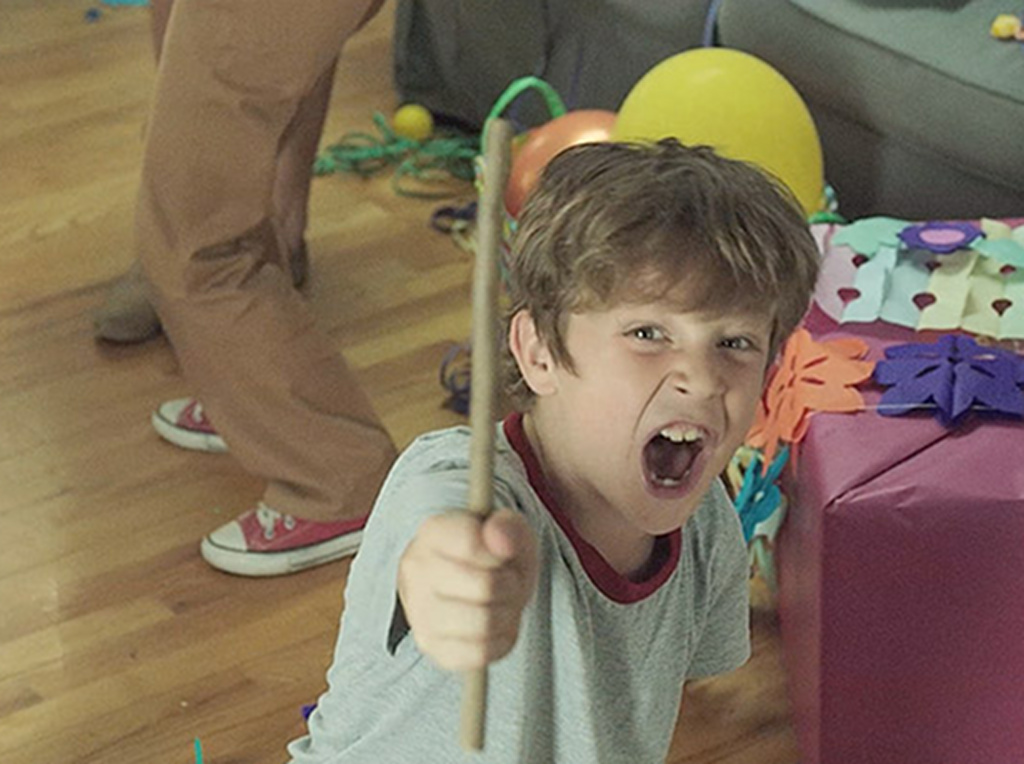
\includegraphics[height=6cm]{pics/un-palo.jpg}
  \end{figure}
\end{frame}

\section{Los últimos diez}

\begin{frame}[fragile]{31. dict.\_\_missing\_\_()}
  \small
  \begin{block}{}
    \centering
    En las \structure{subclases} de dict que definen
    \structure{\_\_missing\_\_()}, el acceso a claves que no estén
    presentes en el diccionario devuelve lo que este método devuelva.
  \end{block}

  \scriptsize
  \begin{exampleblock}{}
    % Escape triple quotes; otherwise string is italicized
    \begin{lstlisting}[escapechar=!]
class MyDict(dict):
    !"""! Diccionario que devuelve -1 si la clave no existe !"""!

    def __missing__(self, key):
        print "'{0}' no encontrado".format(key)
        return -1

>>> d = MyDict()
>>> d[1] = 3
>>> d[1]
3
>>> d[5]
'5' no encontrado
-1
    \end{lstlisting}
  \end{exampleblock}
\end{frame}

\begin{frame}[fragile]{31. dict.\_\_missing\_\_()}
  \small
  \begin{alertblock}{}
    \centering
    \_\_missing\_\_() \structure{no puede ser una variable} -- ha de ser un
    método, que recibirá como argumento la clave que no se ha
    encontrado.
  \end{alertblock}

  \scriptsize
  \begin{exampleblock}
    {\footnotesize Algo que no va a funcionar:}
    \begin{lstlisting}[escapechar=!]
class MyDict(dict):
    !"""! Diccionario que devuelve -1 si la clave no existe !"""!

    __missing__ = -1

>>> d = MyDict()
>>> d[7]
Traceback (most recent call last):
  File "<stdin>", line 1, in <module>
TypeError: 'int' object is not callable
    \end{lstlisting}
  \end{exampleblock}
\end{frame}

\begin{frame}[fragile]{32. collections.defaultdict}
  \small
  \begin{block}{}
    \centering
    Normalmente es mucho mejor, no obstante, usar
    \structure{defaultdict}: se comporta como un diccionario a todos
    con los efectos, con la única diferencia de que al crearlo
    especificamos \structure{el valor que tendrán por defecto} las
    claves a las que accedamos que no existan.
  \end{block}

  \footnotesize
  \begin{exampleblock}
    {Para implementar un contador, en vez de hacer esto...}
    \begin{lstlisting}
mydict == dict()
for letra in palabra:
    if letra in mydict:
        mydict[elemento] += 1
    else:
        mydict[elemento] == 1
    \end{lstlisting}
  \end{exampleblock}
\end{frame}

\begin{frame}[fragile]{32. collections.defaultdict}
  \footnotesize
  \begin{exampleblock}
    {... o incluso esto...}
    \begin{lstlisting}
mydict == dict()
for letra in palabra:
    try:
        mydict[elemento] += 1
    except KeyError:
        pass
    \end{lstlisting}
  \end{exampleblock}
\end{frame}

\begin{frame}[fragile]{32. collections.defaultdict}
  \footnotesize
  \begin{exampleblock}
    {Mucho mejor así:}
    \begin{lstlisting}
import collections
mydict = collections.defaultdict(int)
for letra in palabra:
    mydict[elemento] += 1
    \end{lstlisting}
  \end{exampleblock}

  \small
  \begin{alertblock}{}
    \centering
    ¡Pero esto es sólo un ejemplo! En código real \structure{nunca}
    implementéis un contador así! Lo tenéis ya hecho por gente mucho
    más capaz que nosotros, y disponible desde Python 2.7, en este
    mismo módulo:
    \structure{collections.Counter}.
  \end{alertblock}
\end{frame}

\begin{frame}[fragile]{32. collections.defaultdict}
  \small
  \begin{exampleblock}
    {Valor por defecto: []}
    \begin{lstlisting}
collections.defaultdict(list)
    \end{lstlisting}
  \end{exampleblock}

  \small
  \begin{exampleblock}
    {Valor por defecto: set()}
    \begin{lstlisting}
collections.defaultdict(set)
    \end{lstlisting}
  \end{exampleblock}

  \begin{exampleblock}
    {Valor por defecto: \{\}}
    \begin{lstlisting}
d = collections.defaultdict(dict)
d[0][3] = 3.43
d[1][5] = 1.87
    \end{lstlisting}
  \end{exampleblock}
\end{frame}

\begin{frame}[fragile]{32. collections.defaultdict}
  \small
  \begin{block}{}
    \centering
    Pasar usar valores por defecto \structure{diferentes de cero o
      vacíos}, tenemos que tener presente que lo que
    defaultdict.\_\_init\_\_() recibe es \structure{una función} que
    acepta cero argumentos, que es la que se ejecuta cada vez que la
    clave no se encuentra.
  \end{block}

  \begin{exampleblock}
    {Valor por defecto: -7}
    \begin{lstlisting}
collections.defaultdict(lambda: -7)
    \end{lstlisting}
  \end{exampleblock}

  \begin{exampleblock}
    {Valor por defecto: números [1, 7]}
    \begin{lstlisting}
collections.defaultdict(lambda: range(8))
    \end{lstlisting}
  \end{exampleblock}
\end{frame}

\begin{frame}[fragile]{33. collections.namedtuple}
  \small
  \begin{block}{}
    \centering
    Devuelve un tipo de dato, subclase de \structure{tuple}, que
    podemos usar para crear tuplas que además nos permiten acceder
    también por atributos.  Con \structure{namedtuple} estamos
    definiendo nuestra propia clase en una línea de código -- no deja
    de estar bien, aunque sean clases sencillas.
  \end{block}

  \scriptsize
  \begin{exampleblock}
    {\footnotesize La clase Punto(x, y, z)}
    \begin{lstlisting}
>>> Punto = collections.namedtuple('Punto', ['x', 'y', 'z'])
>>> Punto.__mro__
(<class '__main__.Punto'>, <type 'tuple'>, <type 'object'>
    \end{lstlisting}
  \end{exampleblock}
\end{frame}

\begin{frame}[fragile]{33. collections.namedtuple}
  \small
  \begin{exampleblock}
    {Y ahora usándola:}
    \begin{lstlisting}
>>> dest = Punto(1, 4, 3)
>>> dest.x
1
>>> dest.y
4
>>> dest[2]
3
    \end{lstlisting}
  \end{exampleblock}

  \begin{block}
    {\centering Understanding Python's iterator, iterable, and iteration protocols}
    \centering \url{http://stackoverflow.com/q/9884132/184363}
  \end{block}
\end{frame}

\begin{frame}[fragile]{34. itertools.chain()}
  \small
  \begin{block}{}
    \centering
    La función \structure{chain()}, del módulo \structure{itertools},
    crea un \structure{iterador} que devuelve, uno a uno, elementos de
    cada uno de los iterables que recibe, recorriéndolos todos.
  \end{block}

  \footnotesize
  \begin{exampleblock}{}
    \begin{lstlisting}
>>> import itertools
>>> x = [1, 2, 3]
>>> y = [8, 9, 10]
>>> for numero in itertools.chain(x, y):
...     print numero
...
1
2
3
8
9
10
    \end{lstlisting}
  \end{exampleblock}
\end{frame}

\begin{frame}[fragile]{34. itertools.chain()}
  \scriptsize
  \begin{exampleblock}
    {\footnotesize
      Aplanar una lista de listas, como hicimos antes:}
    \begin{lstlisting}
>>> it = itertools.chain([1, 2], [3], [4, 5], [6, 7, 8])
>>> it
<itertools.chain object at 0x2536590>
>>> list(it)
[1, 2, 3, 4, 5, 6, 7, 8]
>>> list(it)
[]
    \end{lstlisting}
  \end{exampleblock}

  \begin{exampleblock}
  {\footnotesize
    Utilizando * para desempaquetar las sublistas:}
    \begin{lstlisting}
>>> sublistas = [[4, 5], [6, 7]]
>>> list(itertools.chain(*sublistas))
[4, 5, 6, 7]
    \end{lstlisting}
  \end{exampleblock}
\end{frame}

\begin{frame}[fragile]{34. itertools.chain()}
  \small
  \begin{alertblock}{}
    \centering
    Pero \structure{chain()} acepta mucho más que listas: le podemos pasar
    \structure{cualquier cosa sobre la que se pueda iterar}. Esto incluye
    generadores, conjuntos, diccionarios y cualquier objeto cuyos
    elementos podemos recorrer de uno en uno.
  \end{alertblock}

  \scriptsize
  \begin{exampleblock}
    {Dos conjuntos:}
    \begin{lstlisting}
>>> s1 = set([1, 2, 3])
>>> s2 = set([6, 5, 4])
>>> list(itertools.chain(s1, s2))
[1, 2, 3, 4, 5, 6]
    \end{lstlisting}
  \end{exampleblock}

  \begin{exampleblock}
    {Diccionaro (claves) y conjunto:}
    \begin{lstlisting}
>>> d1 = {1 : "uno", 2 : "dos"}
>>> s1 = set(["tres", "cuatro"])
>>> list(itertools.chain(d1, d2))
[1, 2, 'cuatro', 'tres']
    \end{lstlisting}
  \end{exampleblock}
\end{frame}

\begin{frame}[fragile]{35. functools.partial()}
  \small
  \begin{block}{}
    \centering
    En el módulo \structure{functools}, la función
    \structure{partial()} nos permite \emph{congelar} otra función,
    \structure{fijándole argumentos} de forma que podamos llamarla de
    forma más sencilla y corta.
  \end{block}

  \begin{exampleblock}{}
    \begin{lstlisting}
>>> import functools
>>> eleva_dos = functools.partial(pow, 2)
    \end{lstlisting}
  \end{exampleblock}

\begin{exampleblock}
  {Y ahora usándola:}
    \begin{lstlisting}
>>> eleva_dos(3)
8
>>> eleva_dos(10)
1024
    \end{lstlisting}
  \end{exampleblock}
\end{frame}

\begin{frame}[fragile]{35. functools.partial()}
  \small
  \begin{alertblock}{}
    \centering
    Es importante tener presente que los argumentos que nosotros le
    pasamos a la función \emph{congelada} se añaden
    \structure{después} de los que hemos definido en
    \structure{partial()}. Es necesario dar un rodeo si queremos crear
    funciones parciales que añadan los argumentos por el comienzo --
    por ejemplo, para devolver \structure{pow(x, 3)}.
  \end{alertblock}

  \begin{block}
    {\centering Python: Why is functools.partial necessary?}
    \centering \url{http://stackoverflow.com/a/3252425/184363}
  \end{block}

  \begin{block}
    {\centering implementing functools.partial that prepends additional arguments}
    \centering \url{http://stackoverflow.com/q/11831070/184363}
  \end{block}
\end{frame}

\begin{frame}[fragile]{36. Pasando funciones a iter()}
  \begin{block}{}
    \Large
    \centering iter(function, sentinel))
  \end{block}

  \small
  \begin{alertblock}{}
    \centering
    El uso más habitual de \structure{iter()} es pasarle un único
    argumento --- el objeto sobre el que queremos iterar. Pero también
    podemos pasarle una \structure{función}, que es ejecutada una y
    otra vez: en el momento en el que uno de los valores que devuelve
    sea igual a \structure{sentinel}, nos detenemos.
  \end{alertblock}
\end{frame}

\begin{frame}[fragile]{36. Pasando funciones a iter()}
  \small
  \begin{exampleblock}
    {Lee un fichero hasta la primera línea vacía:}
    \begin{lstlisting}
with open('currículum.tex') as fd:
    for linea in iter(fd.readline, '\n'):
        print linea
    \end{lstlisting}
  \end{exampleblock}
\end{frame}

\begin{frame}[fragile]{36. Pasando funciones a iter()}
  \small
  \begin{exampleblock}
    {Genera números aleatorios hasta llegar a cero:}
    \begin{lstlisting}
import random

def aleatorio():
    return random.randint(-10, 10)

for numero in iter(aleatorio, 0):
    print numero
    \end{lstlisting}
  \end{exampleblock}
\end{frame}

\begin{frame}[fragile]{37. Autocompletado en el intérprete}
  \small
  \begin{block}{}
    \centering
    En nuestro fichero \structure{.pythonrc}, estas líneas bastan para
    habilitar el \structure{autocompletado}, que se activa al pulsar
    tabulador, como estamos acostumbrados a hacer en la línea de
    comandos.
  \end{block}

  \begin{exampleblock}{}
    \begin{lstlisting}
import readline
import rlcompleter
readline.parse_and_bind("tab: complete")
    \end{lstlisting}
  \end{exampleblock}

  \footnotesize
  \begin{alertblock}{}
    \centering
    ¡La variable de entorno \structure{PYTHONSTARTUP} debe apuntar a este fichero!
  \end{alertblock}
\end{frame}

\begin{frame}[fragile]{38. Historia de comandos}
  \small
  \begin{block}{}
    \centering
    También podemos habilitar la historia de \structure{todo lo que
      hemos escrito} en el intérprete de Python, accesibles pulsando
    las \structure{teclas de navegación} vertical. Al igual que en una
    terminal cualquiera, la historia se guarda en un fichero, por lo
    que podemos reusar los comandos \structure{de una sesión a otra}.
  \end{block}

  \footnotesize
  \begin{exampleblock}{}
    \begin{lstlisting}
import atexit
import os.path
import readline

history_file = os.path.expanduser('~/.python_history')
if os.path.exists(history_file):
    readline.read_history_file(history_file)
func = readline.write_history_file
atexit.register(func, history_file)
    \end{lstlisting}
  \end{exampleblock}
\end{frame}

\begin{frame}[fragile]{39. Límite de memoria}
  \small
  \begin{block}{}
    \centering
    Antes hemos mencionado que crear una lista de tamaño excesivo
    podría usar \structure{toda la memoria} del ordenador, a veces con
    trágicas consecuencias. Usando esto podemos impedir que Python use
    más del 3/4 de la memoria total de nuestro equipo, abortando la
    ejecución \structure{si sobrepasamos este límite}.
  \end{block}

  \scriptsize
  \begin{exampleblock}{}
    \begin{lstlisting}
def get_ram_size():
    with open('/proc/meminfo', 'rt') as fd:
        regexp = "^MemTotal:\s*(\d+) kB$"
        match = re.match(regexp, fd.read(), re.MULTILINE)
        return int(match.group(1)) * 1024 # kB to bytes
MAX_RAM = get_ram_size() * 0.75
resource.setrlimit(resource.RLIMIT_AS,
                   (MAX_RAM, resource.RLIM_INFINITY))
    \end{lstlisting}
  \end{exampleblock}
\end{frame}

\begin{frame}[fragile]{39. Límite de memoria}
  \footnotesize
  \begin{exampleblock}
    {Esto es lo que ocurre entonces si abarcamos demasiado:}
    \begin{lstlisting}
>>> list(xrange(10e12))
Traceback (most recent call last):
  File ``<stdin>'', line 1, in <module>
MemoryError
    \end{lstlisting}
  \end{exampleblock}

  \small
  \begin{block}
    {\centering Por si alguien quiere reusar mi fichero .pythonrc}
    \centering \url{http://github.com/vterron/dotfiles}
  \end{block}
\end{frame}

\begin{frame}[fragile]{40. a, *b, c = range(5)}
  \begin{exampleblock}
    {\centering Un detalle precioso de Py3K}
    \small
    \begin{lstlisting}[escapechar=!]
>>> primero, !\color{blue}{*resto}! = range(5)
>>> primero
0
>>> resto
[1, 2, 3, 4]
>>> primero, !\color{blue}{*resto}!, ultimo = range(10)
>>> primero
0
>>> resto
[1, 2, 3, 4, 5, 6, 7, 8]
>>> ultimo
9
    \end{lstlisting}
  \end{exampleblock}
\end{frame}

\section{You Are Now a Ninja}
\begin{frame}[fragile]{Programadores Python Shaolín}
  \begin{figure}
    \centering
    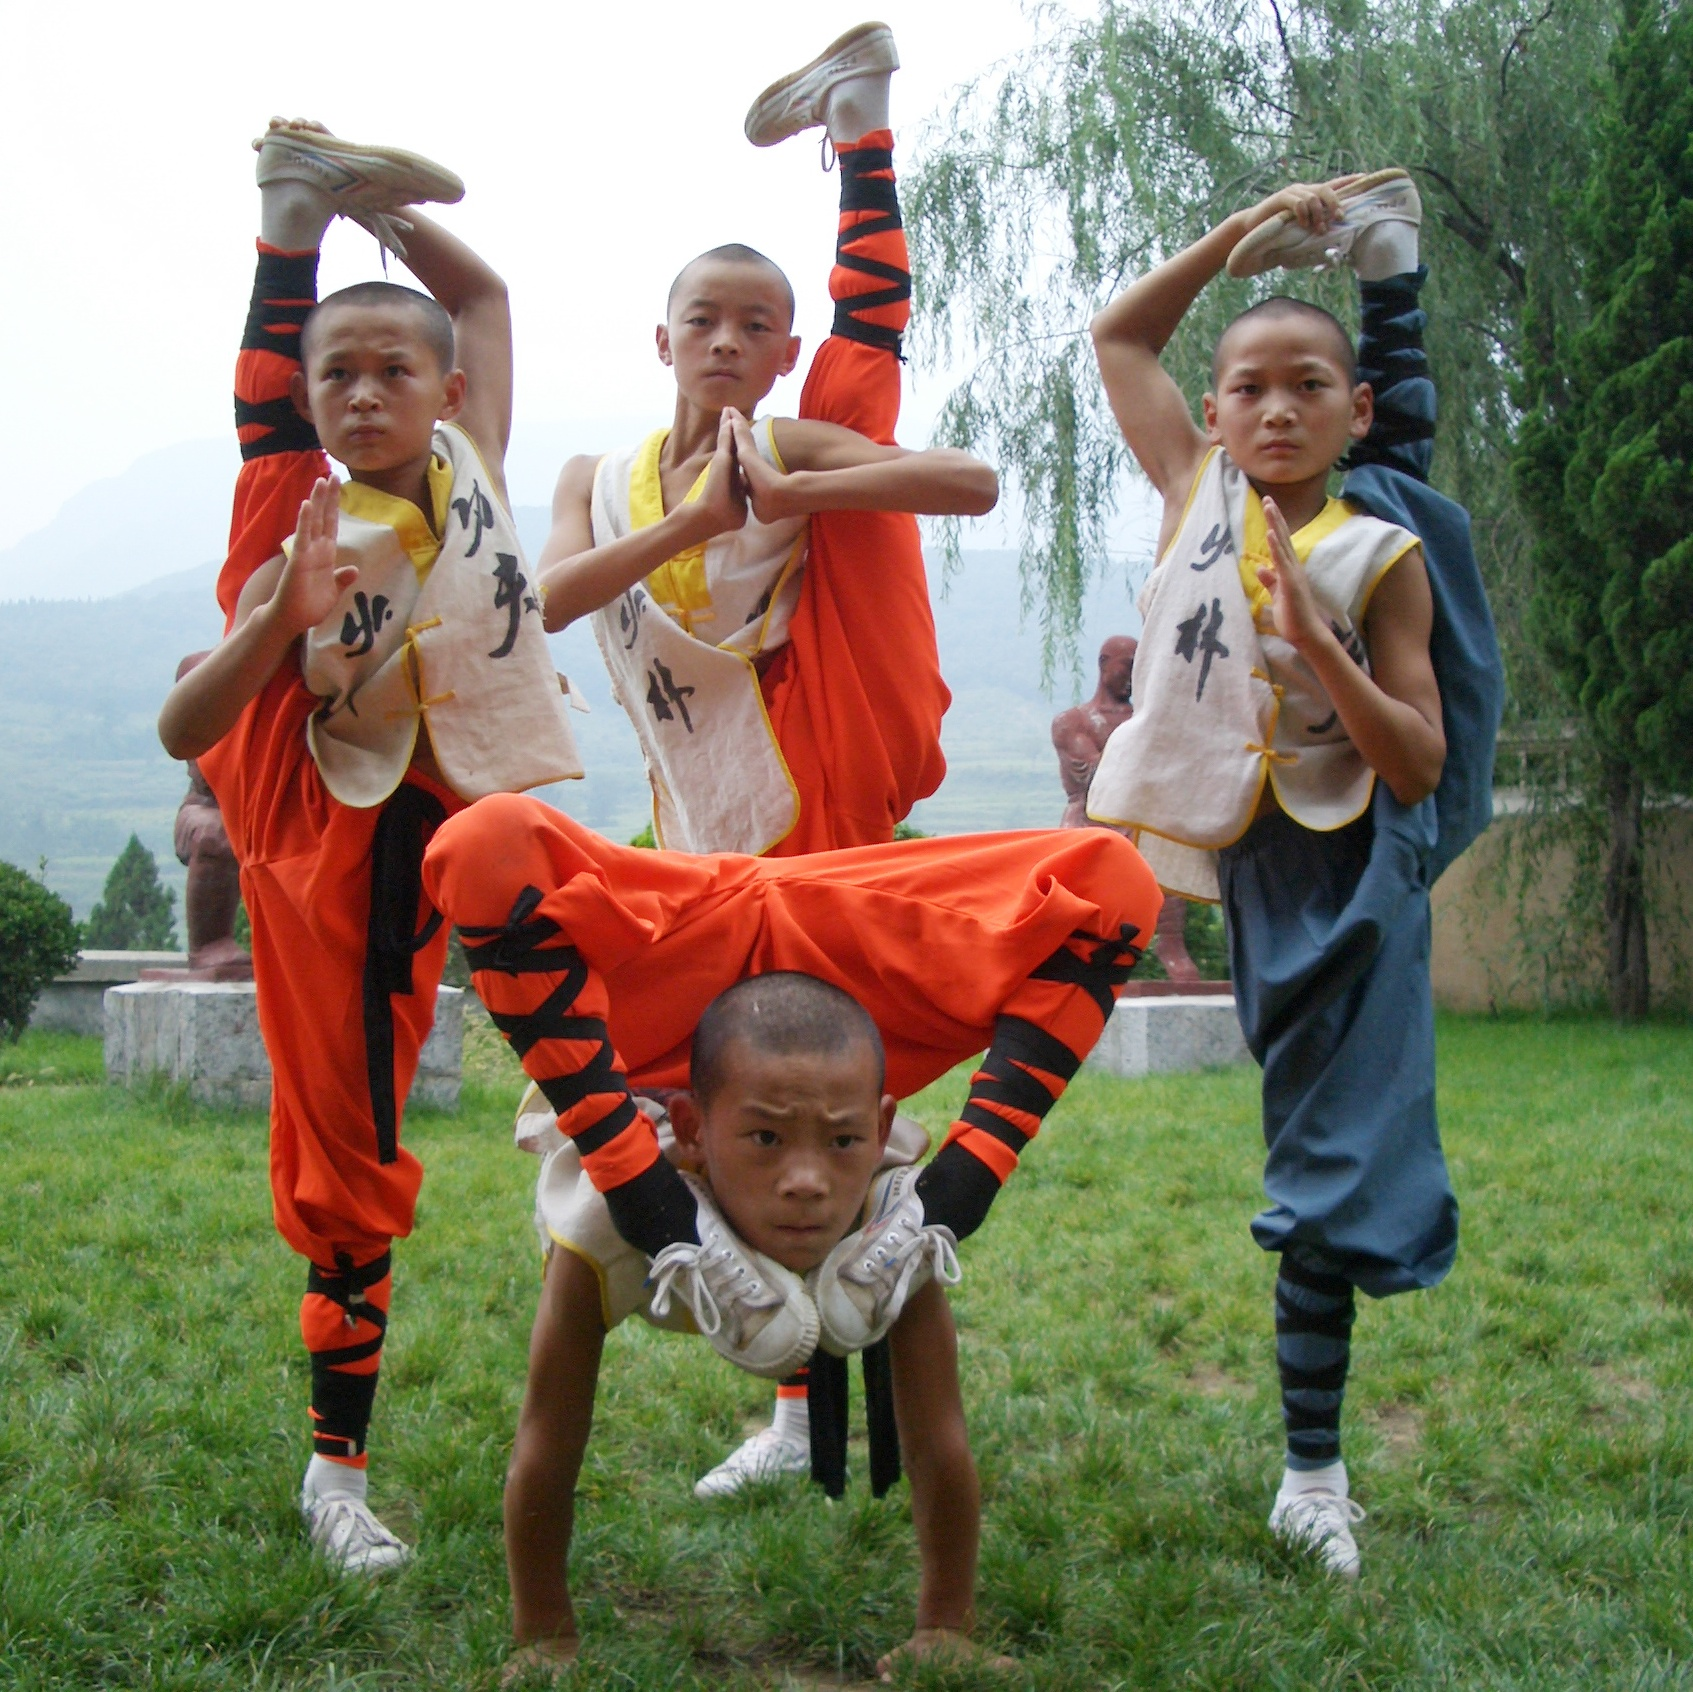
\includegraphics[height=7cm]{pics/shaolin.jpg}
  \end{figure}
\end{frame}

\end{document}
